\section{関手}
  これまで、似たような性質を持つ対象や射を同時に扱う時、それらの対象に添字をつけて量化してきた。対象の量化の例として積対象$A\times B$は圏$\cat{C}$の任意の対象$A$と任意の対象$B$によって添字づけられている。また射の量化の例として、射の積$\mor{f\times g}{\tuple{A,B}}{\tuple{A',B'}}$は圏$\cat{C}$の任意の射$\mor{f}{A}{A'}$、$\mor{g}{B}{B'}$によって添字づけられている。

  この章では主に、この添字づけを行うような操作を圏から圏への特殊な写像である関手で一般化する。

	\begin{define}
		ある圏$\cat{C}$からある圏$\cat{D}$への\textbf{関手}$\functor{F}{C}{D}$は以下の関数と公理から構成される。
		\begin{quote}
			\begin{mydescription}
		\item[対象関数]$\cat{C}$の対象$A$に$\cat{D}$の対象$FA$を割り当てる写像を持つ必要がある。これを\textbf{対象関数}とよび、\[\mor{F}{\obj{C}}{\obj{D}}\]と表すことにする。
		\item[射関数]$\cat{C}$の任意の各対象$A,B$において射$\mor{f}{A}{B}$に圏$\cat{D}$の射$\mor{Ff}{FA}{FB}$を割り当てる写像をそれぞれ持つ必要がある。これを\textbf{射関数}とよび、\[\mor{F_{A,B}}{\arset{C}{A}{B}}{\arset{D}{FA}{FB}}\]と表す。また対象$A,B$に対してそれぞれ存在する射関数$F_{A,B}$を総称して$F$と呼ぶことにする。

		つまり、圏$\cat{C}$に含まれる任意の射$\mor{f}{A}{B}$、$\mor{k}{X}{Y}$に対して\[F(f)=F_{A,B}(f)\]\[F(k)=F_{X,Y}(k)\]と置き換えてほしい。
		また対象関数と射関数は記法で区別しないことと、$Tf,TA$ののように括弧を省略する場合もある。
		\item[恒等射の保存] 射関数は圏$\cat{C}$の恒等射を$\cat{D}$の恒等射に対応させる。つまり$F(id_A)=id_{FA}$が成り立つ。
		\item[射の合成の保存]$\cod(f)=\dom(g)$であるとき、$F(g\circ f)=Fg\circ Ff$が成り立つ。
		\end{mydescription}
		\end{quote}
	\end{define}

  次に関手の具体例を示す。
  以下の射と対象で構成される圏$\cat{C},\cat{D}$と二つの関手$\functor{T}{C}{D}$、$\functor{S}{C}{D}$を考える。
  \begin{center}
    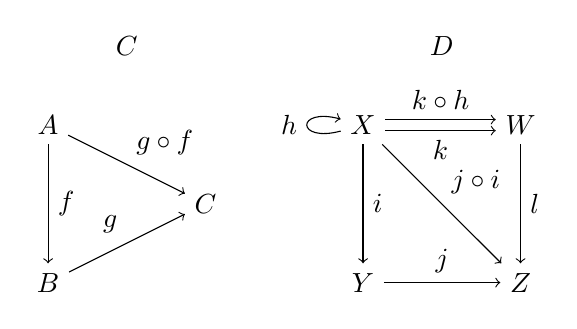
\begin{tikzpicture}[auto]
      \node (a) at (0, 2) {$A$};
      \node (b) at (0, 0) {$B$};
      \node (c) at (2, 1) {$C$};
      \draw[->] (a) to node{$f$}(b);
      \draw[->] (b) to node{$g$}(c);
      \draw[->] (a) to node{$g\circ f$}(c);

      \node (x) at (4, 2) {$X$};
      \node (y) at (4, 0) {$Y$};
      \node (w) at (6, 2) {$W$};
      \node (z) at (6, 0) {$Z$};
      \draw[->] (x) to node{$i$}(y);
      \draw[->] (y) to node{$j$}(z);
      \draw[->] (x) to node{$j\circ i$}(z);
      \draw[->] (w) to node{$l$}(z);
      \draw[->,transform canvas={yshift=-2pt}] (x) to node[swap]{$k$}(w);
      \draw[->,transform canvas={yshift=2pt}] (x) to node{$k\circ h$}(w);
      \draw[->,loop left ,looseness=10] (x) to node{$h$}(x);

      \node (catc) at (1, 3) {$\cat{C}$};
      \node (catd) at (5, 3) {$\cat{D}$};
      %\draw[->,bend right = 15] (catc) to node{$T$}(catd);
      %\draw[->,bend left = 15] (catc) to node{$S$}(catd);
    \end{tikzpicture}
  \end{center}
  そして関手$T$の対象関数$T$を\[T(A)=X,\ T(B)=Y,\ T(C)=Z\]、関手$S$の対象関数$S$を\[S(A)=X,\ S(B)=X,\ S(C)=W\]と定義する。

  次に、関手$T$の射関数$T$を\[T(f)=i,\ T(g)=j,\ T(g\circ f)=j\circ i\]と定義する。また各対象の恒等射の対応は
  \begin{align*}
    T(id_A)&=id_{TA}\\
    &=id_{X}\text{($TA=X$)}\\
    T(id_B)&=id_{TB}\\
    &=id_{Y}\text{($TB=Y$)}\\
    T(id_C)&=id_{TC}\\
    &=id_{Z}\text{($TC=Z$)}
  \end{align*}とする。
  \begin{center}
    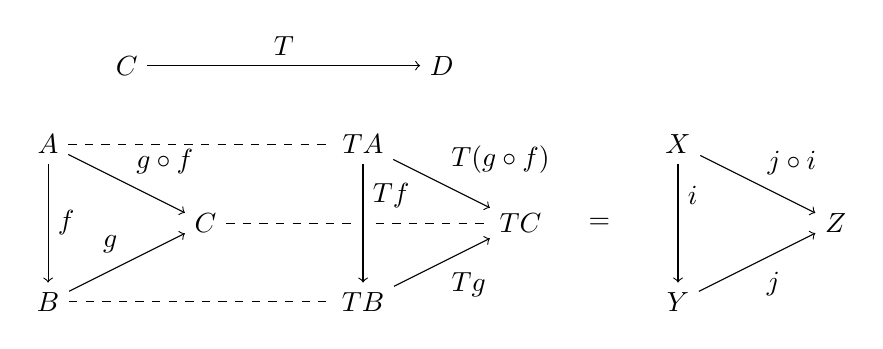
\begin{tikzpicture}[auto]
      \node (a) at (0, 2) {$A$};
      \node (b) at (0, 0) {$B$};
      \node (c) at (2, 1) {$C$};
      \node (ta) at (4, 2) {$TA$};
      \node (tb) at (4, 0) {$TB$};
      \node (tc) at (6, 1) {$TC$};
      \node (x) at (8, 2) {$X$};
      \node (y) at (8, 0) {$Y$};
      \node (z) at (10, 1) {$Z$};

      \node (e) at (7, 1) {$=$};

      \draw[-,dashed] (a) to (ta);
      \draw[-,dashed] (b) to (tb);
      \draw[-,dashed] (c) to (tc);

      \draw[->] (a) to node{$f$}(b);
      \draw[->] (b) to node{$g$}(c);
      \draw[->] (a) to node{$g\circ f$}(c);

      \draw[-, line width=4pt,draw=white] (x) to (y);
      \draw[->] (x) to node[yshift =10]{$i$}(y);
      \draw[->] (y) to node[swap]{$j$}(z);
      \draw[->] (x) to node{$j\circ i$}(z);

      \draw[-, line width=4pt,draw=white] (ta) to (tb);
      \draw[->] (ta) to node[yshift =10]{$Tf$}(tb);
      \draw[->] (tb) to node[swap]{$Tg$}(tc);
      \draw[->] (ta) to node{$T(g\circ f)$}(tc);

      \node (catc) at (1, 3) {$\cat{C}$};
      \node (catd) at (5, 3) {$\cat{D}$};
      \draw[->] (catc) to node{$T$}(catd);

    \end{tikzpicture}
  \end{center}
  この図での点線は対象の写像的な対応を表しているのであって、実際に射が存在するわけではないことに注意してほしい。

  同様に関手$S$の射関数$S$を\[S(f)=h,\ S(g)=k,\ S(g\circ f)=k\circ h\]と定義する。
  恒等射の対応は
  \begin{align*}
    S(id_A)&=id_{SA}\\
    &=id_{X}\text{($SA=X$)}\\
    S(id_B)&=id_{SB}\\
    &=id_{X}\text{($SB=X$)}\\
    S(id_C)&=id_{SC}\\
    &=id_{W}\text{($SC=W$)}
  \end{align*}
  とする。
  \begin{center}
    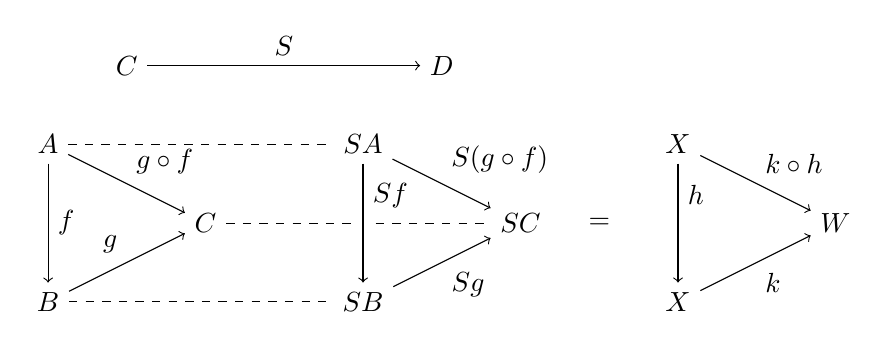
\begin{tikzpicture}[auto]
      \node (a) at (0, 2) {$A$};
      \node (b) at (0, 0) {$B$};
      \node (c) at (2, 1) {$C$};
      \node (ta) at (4, 2) {$SA$};
      \node (tb) at (4, 0) {$SB$};
      \node (tc) at (6, 1) {$SC$};
      \node (x) at (8, 2) {$X$};
      \node (y) at (8, 0) {$X$};
      \node (z) at (10, 1) {$W$};

      \node (e) at (7, 1) {$=$};

      \draw[-,dashed] (a) to (ta);
      \draw[-,dashed] (b) to (tb);
      \draw[-,dashed] (c) to (tc);

      \draw[->] (a) to node{$f$}(b);
      \draw[->] (b) to node{$g$}(c);
      \draw[->] (a) to node{$g\circ f$}(c);

      \draw[-, line width=4pt,draw=white] (x) to (y);
      \draw[->] (x) to node[yshift =10]{$h$}(y);
      \draw[->] (y) to node[swap]{$k$}(z);
      \draw[->] (x) to node{$k\circ h$}(z);

      \draw[-, line width=4pt,draw=white] (ta) to (tb);
      \draw[->] (ta) to node[yshift =10]{$Sf$}(tb);
      \draw[->] (tb) to node[swap]{$Sg$}(tc);
      \draw[->] (ta) to node{$S(g\circ f)$}(tc);

      \node (catc) at (1, 3) {$\cat{C}$};
      \node (catd) at (5, 3) {$\cat{D}$};
      \draw[->] (catc) to node{$S$}(catd);
    \end{tikzpicture}
  \end{center}

  関手$S$、$T$が恒等射を保つことは恒等射の定義から用意に分かる。また、恒等射の合成は省略するが、射の合成の保存は
  \begin{align*}
    T(g\circ f)&=j\circ i&\text{($T(g\circ f)$の定義)}\\
    &=Tg\circ Tf&\text{($Tg,Tf$の定義)}\\
    S(g\circ f)&=k\circ h&\text{($S(g\circ f)$の定義)}\\
    &=Sg\circ Sf&\text{($Sg,Sf$の定義)}
  \end{align*}
  が成り立つことから分かる。

  関手$T$の例で言えば、圏$\cat{D}$の対象$X$は$TA$として圏$\cat{C}$の対象$A$によって添字付けられた対象であると考えられる。また、$X$は別の関手$S$によって$SA,SB$として添字付けられていると考えることもできる。

	\begin{define}[関手の同一性]
		関手$\functor{F,G}{C}{D}$が\textbf{同一}、$F=G$であるとは、それぞれの対象関数、射関数が写像として等しいということである。
	\end{define}


	\begin{prop}[図式の圏論的な定義]
		添字圏と呼ばれる圏$\cat{J}$から図式を取りたい圏$\cat{C}$への関手は図式である。
		例えば以下のように対象$I,J,K$と射$i,j$で構成される添字圏$J$を図式の骨組み、関手$\functor{F}{I}{C}$を図式の骨組みに圏$C$の対象と射を割り当てる操作とする。

		すると関手の合成の保存より、図式中の射$f,g$の合成射$g\circ f$は図式に必ず存在する。
    また恒等射の保存より、図式中の対象に必ず恒等射となる射が存在し、関手の合成の保存により実際に恒等射のように振る舞う。

    このように関手の性質によって、図式はそれ単体で圏のように振る舞う。
		\begin{center}
			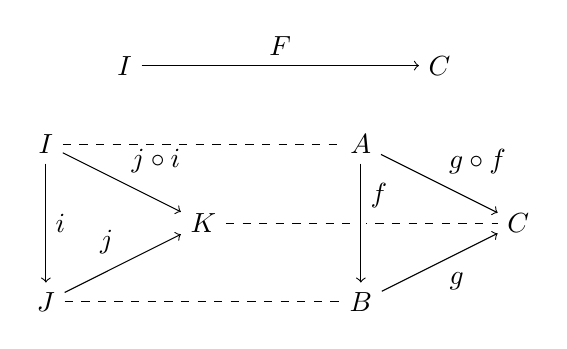
\begin{tikzpicture}[auto]
				\node (a) at (0, 2) {$I$};
				\node (b) at (0, 0) {$J$};
				\node (c) at (2, 1) {$K$};
				\node (x) at (4, 2) {$A$};
				\node (y) at (4, 0) {$B$};
				\node (z) at (6, 1) {$C$};
				\draw[-,dashed] (a) to (x);
				\draw[-,dashed] (b) to (y);
				\draw[-,dashed] (c) to (z);

				\draw[->] (a) to node{$i$}(b);
				\draw[->] (b) to node{$j$}(c);
				\draw[->] (a) to node{$j\circ i$}(c);

				\draw[-, line width=4pt,draw=white] (x) to (y);
				\draw[->] (x) to node[yshift =10]{$f$}(y);
				\draw[->] (y) to node[swap]{$g$}(z);
				\draw[->] (x) to node{$g\circ f$}(z);
				\node (catc) at (1, 3) {$\cat{I}$};
				\node (catd) at (5, 3) {$\cat{C}$};
				\draw[->] (catc) to node{$F$}(catd);

			\end{tikzpicture}
		\end{center}
	\end{prop}
  次に最初に述べた積対象$A\times B$の添字づけについて実際に関手で定式化する。
  ただし、積対象$A\times B$は二つの対象$A,B$によって添字付けられているが、今回は対象$A$にだけを量化し、対象$B$を固定して考える。
	\begin{define}[積関手]
		圏$\cat{C}$が積を持つとき、以下の関数で構成されるある対象$B$に対して圏$C$から圏$C$への関手$\functor{-\times B}{C}{C}$を\textbf{積関手}と呼ぶ。
		\begin{quote}
			\begin{mydescription}
			\item[対象関数] 対象関数を$(-\times B)(A)=A\times B$と定義する。
			\item[射関数] 圏$C$の任意の対象$A,A'$に対する関数$(-\times B)_{A,A'}$を任意の射$\mor{f}{A}{A'}$に対して
			\begin{align*}
				(-\times B)_{A,A'}(f)&=\mor{f\times id_B}{(-\times B)(A)}{(-\times B)(A)}\\
				&=\mor{f\times id_B}{A\times B}{A'\times B}
			\end{align*}
			と定義する。同様に任意の対象$A,A'$に対して存在する射関数$(-\times B)_{A,A'}$を総称して$(-\times B)$と呼ぶ。
			\begin{center}
				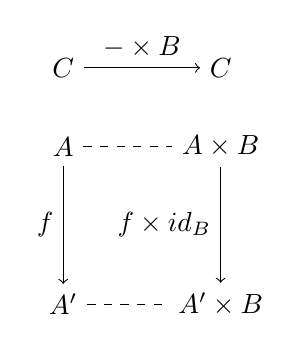
\begin{tikzpicture}[auto]
					\node (a) at (0, 2) {$A$};
					\node (a') at (0, 0) {$A'$};
					\node (ab) at (2, 2) {$A\times B$};
					\node (a'b) at (2, 0) {$A'\times B$};
					\node (catc1) at (0, 3) {$\cat{C}$};
					\node (catc2) at (2, 3) {$\cat{C}$};
					\draw[-,dashed] (a) to (ab);
					\draw[-,dashed] (a') to (a'b);

					\draw[->] (catc1) to node{$-\times B$}(catc2);
					\draw[->] (a) to node[swap]{$f$}(a');
					\draw[->] (ab) to node[swap]{$f\times id_B$}(a'b);
				\end{tikzpicture}
			\end{center}
			\item[恒等射の保存] 射影射の対が恒等射になることを用いて$(-\times B)(id_A)=id_{(-\times B)(A)}$を示せばよい。
			\begin{align*}
				(-\times B)(id_A)&=id_A\times id_B&\text{(射関数の定義)}\\
				&=\tuple{id_A\circ\pi_A,id_B\circ\pi_B}&\text{(射の積の定義)}\\
				&=\tuple{\pi_A,\pi_B}&\text{(恒等射の性質)}\\
				&=id_{A\times B}&\text{(射影射の対)}\\
				&=id_{(-\times B)(A)}&\text{(対象関数の定義)}
			\end{align*}
			よって積関手は恒等射を保つことが示せた。
			\item[射の合成の保存]任意の対象$A,A',A''$と任意の射$\mor{f}{A}{A'},\mor{f'}{A'}{A''}$に対して\[(-\times B)(f'\circ f)=(-\times B)(f')\circ(-\times B)(f)\]が成り立つことを、積と合成の交換から示す。
			\begin{align*}
				(-\times B)(f'\circ f)&=(f'\circ f)\times id_B&\text{(射関数の定義)}\\
				&=(f'\circ f)\times (id_B\circ id_B)&\text{(恒等射の性質)}\\
				&=(f'\times id_B)\circ(f\times id_B)&\text{(積と合成の交換)}\\
				&=(-\times B)(f')\circ(-\times B)(f)&\text{(射関数の定義)}
			\end{align*}
			\begin{center}
				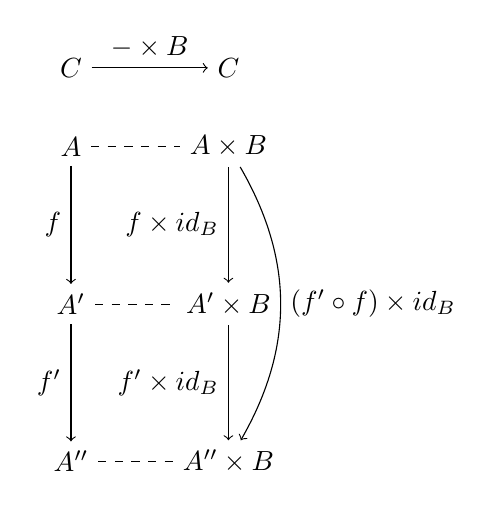
\begin{tikzpicture}[auto]
					\node (a) at (0, 2) {$A$};
					\node (a') at (0, 0) {$A'$};
					\node (a'') at (0, -2) {$A''$};
					\node (ab) at (2, 2) {$A\times B$};
					\node (a'b) at (2, 0) {$A'\times B$};
					\node (a''b) at (2, -2) {$A''\times B$};
					\node (catc1) at (0, 3) {$\cat{C}$};
					\node (catc2) at (2, 3) {$\cat{C}$};
					\draw[-,dashed] (a) to (ab);
					\draw[-,dashed] (a') to (a'b);
					\draw[-,dashed] (a'') to (a''b);
					\draw[->] (catc1) to node{$-\times B$}(catc2);
					\draw[->] (a) to node[swap]{$f$}(a');
					\draw[->] (a') to node[swap]{$f'$}(a'');
					\draw[->] (ab) to node[swap]{$f\times id_B$}(a'b);
					\draw[->] (a'b) to node[swap]{$f'\times id_B$}(a''b);
					\draw[->,bend left =30] (ab) to node{$(f'\circ f)\times id_B$}(a''b);
				\end{tikzpicture}
			\end{center}
			よって積関手は射の合成を保つことが示せた。
		\end{mydescription}
		\end{quote}
	\end{define}
	\begin{prop}[関手の同型の保存]
		任意の圏$\cat{C,D}$と任意の関手$\functor{F}{C}{D}$、圏$\cat{C}$の対象$A,B$において、
		\[A\cong B \Longrightarrow FA\cong FB\]が成り立つ。
	\end{prop}
	\begin{proof}
		同型$A\cong B$のある同型射$\mor{i}{A}{B},\mor{i^{-1}}{B}{A}$に対して$\mor{Fi}{FA}{FB},\mor{Fi^{-1}}{FB}{FA}$も同様に同型射であることを示せばよい。

		\begin{align*}
			Fi^{-1}\circ Fi&=F(i^{-1}\circ i)&\text{($F$の射の合成の保存)}\\
			&=F(id_A)&\text{(恒等射の定義)}\\
			&=id_{FA}&\text{($F$の恒等射の保存)}\\
			Fi\circ Fi^{-1}&=F(i\circ i^{-1})&\text{($F$の射の合成の保存)}\\
			&=F(id_B)&\text{(恒等射の定義)}\\
			&=id_{FB}&\text{($F$の恒等射の保存)}\\
		\end{align*}
		$Fi^{-1}\circ Fi=id_{FA}$、$Fi\circ Fi^{-1}=id_{FB}$より、$Fi,Fi^{-1}$が同型射なる。
		よって$FA\cong FB$が成り立つ。
	\end{proof}
  一般に逆は成り立たないことに注意してほしい。
	\subsection{小さい圏の圏}
	関手は圏から圏への一種の写像であるため、集合の圏のように、圏を対象とし関手を射とするような圏である圏の圏を考えることができそうである。
	そのためにもまずは合成射、恒等射にあたる関手を定義していく。
	\begin{define}[合成関手]
		関手$\functor{F}{C}{C'}$、$\functor{G}{C'}{C''}$を合成した関手$\functor{G\circ F}{C}{C'}$を以下の要素によって定義する。
		\begin{quote}
			\begin{mydescription}
			\item[対象関数]関手$F,G$のそれぞれの対象関数$F,G$に対して$G\circ F$の対象関数を$G\circ F$と定義する。つまり圏$\cat{C}$の任意の対象$A$に対して\[(G\circ F)(A)=G(FA)\]となるような写像である。
			\item[射関数]関手$F,G$のそれぞれの射関数$F,G$に対して$G\circ F$の射関数を$G\circ F$と定義する。
			つまり圏$\cat{C}$の任意の対象$A,A'$と任意の射$\mor{f}{A}{A'}$に対して\[\mor{(G\circ F)_{}(f)=G(Ff)}{GFA}{GF{A'}}\]となるような写像である。

			各二対象ごとの射関数も見ていくと、関手$F,G$のそれぞれの関数\[\mor{F_{A,A'}}{\arset{C}{A}{A'}}{\arset{C'}{FA}{FA'}}\]\[\mor{G_{FA,FA'}}{\arset{C'}{FA}{FA'}}{\arset{C''}{GFA}{GFA'}}\]に対して$G\circ F$の関数を\[(G\circ F)_{A,A'}=\mor{G_{FA,FA'}\circ F_{A,A'}}{\arset{C}{A}{A'}}{\arset{C''}{GFA}{GFA'}}\]となる。このように関手の合成はそれぞれの関手の対象関数、射関数の合成に還元して考える。

			\begin{center}
				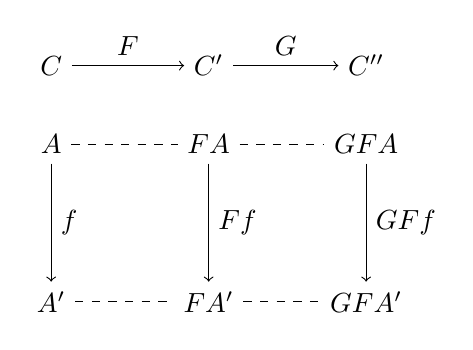
\begin{tikzpicture}[auto]
					\node (a) at (0, 2) {$A$};
					\node (a') at (0, 0) {$A'$};
					\node (fa) at (2, 2) {$FA$};
					\node (fa') at (2, 0) {$FA'$};
					\node (gfa) at (4, 2) {$GFA$};
					\node (gfa') at (4, 0) {$GFA'$};
					\node (catc) at (0, 3) {$\cat{C}$};
					\node (catc') at (2, 3) {$\cat{C'}$};
					\node (catc'') at (4, 3) {$\cat{C''}$};
					\draw[-,dashed] (a) to (fa);
					\draw[-,dashed] (a') to (fa');
					\draw[-,dashed] (fa) to (gfa);
					\draw[-,dashed] (fa') to (gfa');
					\draw[->] (catc) to node{$F$}(catc');
					\draw[->] (catc') to node{$G$}(catc'');

					\draw[->] (a) to node{$f$}(a');
					\draw[->] (fa) to node{$Ff$}(fa');
					\draw[->] (gfa) to node{$GFf$}(gfa');

				\end{tikzpicture}
			\end{center}
			また紛らわしくない場合は合成関手$G\circ F$を$GF$と略すことにする。
			\item[恒等射の保存] $GF(id_A)=id_{GFA}$を示せばよい。
				\begin{align*}
					GF(id_A)&=G(F(id_A))&\text{(射関数の定義)}\\
					&=G(id_{FA})&\text{(関手$F$の恒等射の保存)}\\
					&=id_{GFA}&\text{(関手$G$の恒等射の保存)}
				\end{align*}
			よって合成関手は恒等射を保つ。
			\item[射の合成の保存] $GF(g\circ f)=GFg\circ GFf$を示せばよい。
				\begin{align*}
					GF(g\circ f)&=G(F(g\circ f))&\text{(射関数の定義)}\\
					&=G(Fg\circ Ff)&\text{(関手$F$の射の合成の保存)}\\
					&=GFg\circ GFf&\text{(関手$G$の射の合成の保存)}
				\end{align*}
			よって合成関手は射の合成を保つ。
			\begin{center}
				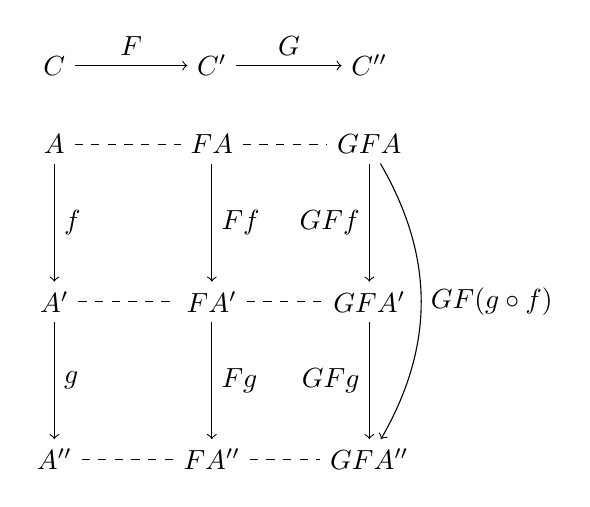
\begin{tikzpicture}[auto]
					\node (a) at (0, 2) {$A$};
					\node (a') at (0, 0) {$A'$};
					\node (a'') at (0, -2) {$A''$};
					\node (fa) at (2, 2) {$FA$};
					\node (fa') at (2, 0) {$FA'$};
					\node (fa'') at (2, -2) {$FA''$};
					\node (gfa) at (4, 2) {$GFA$};
					\node (gfa') at (4, 0) {$GFA'$};
					\node (gfa'') at (4, -2) {$GFA''$};
					\node (catc) at (0, 3) {$\cat{C}$};
					\node (catc') at (2, 3) {$\cat{C'}$};
					\node (catc'') at (4, 3) {$\cat{C''}$};
					\draw[-,dashed] (a) to (fa);
					\draw[-,dashed] (a') to (fa');
					\draw[-,dashed] (a'') to (fa'');
					\draw[-,dashed] (fa) to (gfa);
					\draw[-,dashed] (fa') to (gfa');
					\draw[-,dashed] (fa'') to (gfa'');
					\draw[->] (catc) to node{$F$}(catc');
					\draw[->] (catc') to node{$G$}(catc'');

					\draw[->] (a) to node{$f$}(a');
					\draw[->] (a') to node{$g$}(a'');

					\draw[->] (fa) to node{$Ff$}(fa');
					\draw[->] (fa') to node{$Fg$}(fa'');

					\draw[->] (gfa) to node[swap]{$GFf$}(gfa');
					\draw[->] (gfa') to node[swap]{$GFg$}(gfa'');
					\draw[->,bend left =30] (gfa) to node{$GF(g\circ f)$}(gfa'');
				\end{tikzpicture}
			\end{center}
		\end{mydescription}
		\end{quote}
	\end{define}
	\begin{define}[恒等関手]
		任意の圏$\cat{C}$の\textbf{恒等関手}$\functor{Id_{\cat{C}}}{C}{C}$を以下の要素で定義する。
		\begin{quote}
			\begin{mydescription}
				\item[対象関数] 対象関数を恒等写像$Id_{\cat{C}}(A)=A$と定義する。
				\item[射関数] 射関数を恒等写像$Id_{\cat{C}}(f)=f$と定義する。
				\item[恒等射の保存] $Id_{\cat{C}}(id_C)=id_C=id_{Id_{\cat{C}}(C)}$より恒等射を保つ
				\item[射の合成の保存] $Id_{\cat{C}}(g\circ f)=g\circ f=Id_{\cat{C}}(g)\circ Id_{\cat{C}}(f)$より射の合成を保つ。
			\end{mydescription}
		\end{quote}
	\end{define}
	\begin{define}[小さい圏の圏]
		\textbf{小さい圏の圏}$\cat{Cat}$は以下の要素で構成される。

		集合の圏の時と同様に、小さい圏の「小さい」とは簡単に説明をするのであれば自己言及を防ぐための条件付けであり、実際に$\cat{Cat}$は小さい圏ではないため$\cat{Cat}$の対象にはならない。
		\begin{quote}
			\begin{mydescription}
				\item[対象] 任意の小さい圏
				\item[射] 任意の小さい圏$\cat{A,B}$の間の任意の関手$\functor{F}{A}{B}$
				\item[射の合成] 関手$\functor{F}{C}{C'}$、$\functor{G}{C'}{C''}$に対して合成した関手$\functor{G\circ F}{C}{C'}$をとる操作を射の合成とする。
				\item[恒等射の存在]任意の圏$\cat{A}$の恒等関手$Id_{\cat{A}}$を恒等射とする。
				\item[結合律]
				$H\circ (G\circ F)=(H\circ G)\circ F$が合成可能な任意の関手$F,G,H$で成り立つことを示せばよい。
				二つの関手が等しいことを示すにはそれぞれを構成する対象関数と射関数が等しいことを示せばよい。
				対象関数については、関手$F,G,H$の対象関数$F,G,H$に対して$H\circ (G\circ F)=(H\circ G)\circ F$は明らかに成り立つ。
				射関数についても写像の結合律に還元すると、
				\begin{align*}
					(H\circ (G\circ F))_{A,A'}&=H_{GFA,GFA'}\circ (G\circ F)_{A,A}&\text{(射関数の合成の定義)}\\
					&=H_{GFA,GFA'}\circ (G_{FA,FA'}\circ F_{A,A'})&\text{(射関数の合成の定義)}\\
					&=(H_{GFA,GFA'}\circ G_{FA,FA'})\circ F_{A,A'}&\text{(写像の結合則)}\\
					&=(H\circ G)_{FA,FA'}\circ F_{A,A'}&\text{(射関数の合成の定義)}\\
					&=(H\circ (G\circ F))_{A,A'}&\text{(射関数の合成の定義)}
				\end{align*}
				となり、射関数においても結合則が成り立つ。
				\item[単位元律]
				任意の圏$\cat{C}$の恒等関手$Id_{\cat{C}}$と任意の関手$\functor{F}{X}{C}$、$\functor{G}{C}{Y}$において$Id_{\cat{C}}\circ F=F$、$G\circ Id_{\cat{C}}=G$が成り立つことを示せばよい。

				恒等関手の対象関数、射関数ともに恒等写像
				\[\mor{Id_\cat{C}=id_{\obj{A}}}{\obj{A}}{\obj{A}}\]
				\[\mor{Id_{\cat{C}A,A'}=id_{\arset{C}{A}{A'}}}{\arset{C}{A}{A'}}{\arset{C}{A}{A'}}\]
				となるため、写像の単位元律より$Id_{\cat{C}}\circ F=F$、$G\circ Id_{\cat{C}}=G$が成り立ち単位元律が成り立つ。
			\end{mydescription}
		\end{quote}
	\end{define}
	\subsection{積圏と一点離散圏}
  一般的に圏は対象の集合や射集合を具体的な元を指定することで定義して、それが公理を満たすか確認していたが、すでに集合や写像は圏論的な操作で扱うことができる。そのため、これから$\cat{Cat}$における積対象となる積圏と、終対象となる一点離散圏、その周辺の関手を集合の圏を用いて定義していく。
	\begin{define}[積圏]
		ある圏$\cat{A,B}$に対する\textbf{積圏}$\cat{A\times B}$を以下の要素で定義する。
		\begin{quote}
			\begin{mydescription}
				\item[対象] \[\obj{A\times B}=\obj{A}\times\obj{B}\]
				すなわち、圏$\cat{A}$と圏$\cat{B}$の任意の対象$A,B$の対$\tuple{A,B}$が$\cat{A\times B}$の対象であり、紛らわしくないように\[\tuple{A,B}=\pcobj{A,B}\]と表記する。

				また$\obj{A}\times\obj{B}$は直積集合であり、集合の圏の積対象であるが、圏$\cat{A\times B}$の対象$\pcobj{A,B}$そのものは積の普遍性を持たないことに注意してほしい。今回積とみなすのは対象ではなく圏の方である。
				\item[射]任意の対象$\pcobj{A,B},\pcobj{A',B'}$に対してその射集合をそれぞれ\[\arset{(A\times B)}{\pcobj{A,B}}{\pcobj{A',B'}}=\arset{A}{A}{A'}\times\arset{B}{B}{B'}\]と定義する。

				すなわち、圏$\cat{A}$の射$\mor{f}{A}{A'}$と圏$\cat{B}$の射$\mor{g}{B}{B'}$の元の対\[\mor{\tuple{f,g}}{[A,B]}{[A',B']}\]が$\cat{A\times B}$の射であり、対象と同様に\[\tuple{f,g}=\pcobj{f,g}\]と表記する。射の対と同じ表記であるが、対象の表記と同様に積の普遍性は持たないため射の対ではない。
				同様に$\arset{A}{A}{A'}\times\arset{B}{B}{B'}$も直積集合であり、集合の圏の積対象である。
				\begin{center}
					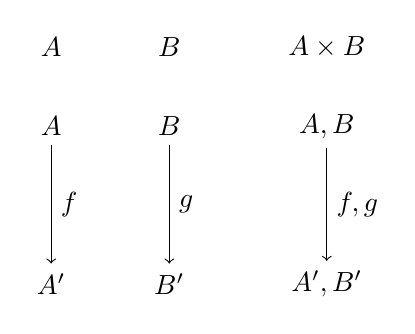
\begin{tikzpicture}[auto]
						\node (a) at (0, 0) {$A$};
						\node (a') at (0, -2) {$A'$};
						\node (b) at (1.5, 0) {$B$};
						\node (b') at (1.5, -2) {$B'$};
						\node (ab) at (3.5, 0) {$\pcobj{A,B}$};
						\node (ab') at (3.5, -2) {$\pcobj{A',B'}$};
						\draw[->] (a) to node{$f$}(a');
						\draw[->] (b) to node{$g$}(b');
						\draw[->] (ab) to node{$\pcobj{f,g}$}(ab');
						\node (cata) at (0, 1) {$\cat{A}$};
						\node (catb) at (1.5, 1) {$\cat{B}$};
						\node (catb) at (3.5, 1) {$\cat{A\times B}$};
					\end{tikzpicture}
				\end{center}
				\item[射の合成] 射$\mor{\pcobj{f,g}}{\pcobj{A,B}}{\pcobj{A',B'}}$と$\mor{\pcobj{f',g'}}{\pcobj{A',B'}}{\pcobj{A'',B''}}$の合成射\[\mor{\pcobj{f',g'}\circ\pcobj{f,g}}{\pcobj{A,B}}{\pcobj{A',B'}}\]を\[\pcobj{f',g'}\circ\pcobj{f,g}=\pcobj{f'\circ f,g'\circ g}\]と定義する。
				\begin{center}
					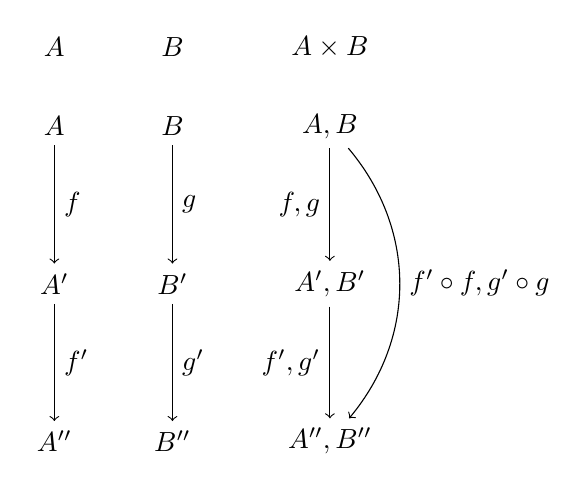
\begin{tikzpicture}[auto]
						\node (a) at (0, 0) {$A$};
						\node (a') at (0, -2) {$A'$};
						\node (a'') at (0, -4) {$A''$};
						\node (b) at (1.5, 0) {$B$};
						\node (b') at (1.5, -2) {$B'$};
						\node (b'') at (1.5, -4) {$B''$};
						\node (ab) at (3.5, 0) {$\pcobj{A,B}$};
						\node (ab') at (3.5, -2) {$\pcobj{A',B'}$};
						\node (ab'') at (3.5, -4) {$\pcobj{A'',B''}$};
						\draw[->] (a) to node{$f$}(a');
						\draw[->] (a') to node{$f'$}(a'');
						\draw[->] (b) to node{$g$}(b');
						\draw[->] (b') to node{$g'$}(b'');
						\draw[->] (ab) to node[swap]{$\pcobj{f,g}$}(ab');
						\draw[->] (ab') to node[swap]{$\pcobj{f',g'}$}(ab'');
						\draw[->,bend left =40] (ab) to node{$\pcobj{f'\circ f,g'\circ g}$}(ab'');
						\node (cata) at (0, 1) {$\cat{A}$};
						\node (catb) at (1.5, 1) {$\cat{B}$};
						\node (catb) at (3.5, 1) {$\cat{A\times B}$};
					\end{tikzpicture}
				\end{center}
				\item[恒等射の存在] 対象$[A,B]$の恒等射$id_{\pcobj{A,B}}$を\[id_{\pcobj{A,B}}=\pcobj{id_A,id_B}\]と定義する。
				\item[結合律]$(\pcobj{f'',g''}\circ\pcobj{f',g'})\circ\pcobj{f,g}=\pcobj{f'',g''}\circ(\pcobj{f',g'}\circ\pcobj{f,g})$を示せばよい。積圏の射の合成の定義を用いて圏の結合律に還元する。
				\begin{align*}
					(\pcobj{f'',g''}\circ\pcobj{f',g'})\circ\pcobj{f,g}&=\pcobj{(f''\circ f')\circ f,(g''\circ g')\circ g}&\text{(積圏の射の合成の定義)}\\
					&=\pcobj{f''\circ (f'\circ f),g''\circ (g'\circ g)}&\text{(圏$\cat{A,B}$の結合則)}\\
					&=\pcobj{f'',g''}\circ(\pcobj{f',g'}\circ\pcobj{f,g})&\text{(積圏の射の合成の定義)}
				\end{align*}
				よって成り立つ。
				\item[単位元律]任意の対象$\pcobj{A,B}$と恒等射$id_{\pcobj{A,B}}$、任意の射$\mor{\pcobj{f,g}}{\pcobj{X,Y}}{\pcobj{A,B}}$、$\mor{\pcobj{f',g'}}{\pcobj{A,B}}{\pcobj{X',Y'}}$において\[id_{\pcobj{A,B}}\circ\pcobj{f,g}=\pcobj{f,g}],\ \pcobj{f',g'}\circ id_{\pcobj{A,B}}=\pcobj{f',g'}\]が成り立つことを示せばよい。同様に積圏の射の合成の定義を用いて圏の結合律に還元する。
				\begin{align*}
					id_{\pcobj{A,B}}\circ\pcobj{f,g}&=\pcobj{id_A,id_B}\circ\pcobj{f,g}&\text{(圏$\cat{A\times B}$の恒等射の定義)}\\
					&=\pcobj{id_A\circ f,id_B\circ g}&\text{(圏$\cat{A\times B}$の射の合成の定義)}\\
					&=\pcobj{f,g}&\text{(圏$\cat{A,B}$の単位元律)}\\
					\pcobj{f',g'}\circ id_{\pcobj{A,B}}&=\pcobj{f',g'}\circ\pcobj{id_A,id_B}&\text{(圏$\cat{A\times B}$の恒等射の定義)}\\
					&=\pcobj{f'\circ id_A,g'\circ id_B}&\text{(圏$\cat{A\times B}$の射の合成の定義)}\\
					&=\pcobj{f',g'}&\text{(圏$\cat{A,B}$の単位元律)}
				\end{align*}
				よって単位元律が成り立つ。
			\end{mydescription}
		\end{quote}
	\end{define}


	\begin{define}[射影関手]
		\textbf{射影関手}$\functor{\Pi_{L,\cat{A\times B}}}{A\times B}{A}$を以下の写像で定義する。また射影射と同様に紛らわしくない場合に$\Pi_{L,\cat{A\times B}}=\Pi_\cat{A}$と表記する。
		\begin{quote}
			\begin{mydescription}
				\item[対象関数] 積圏の対象の定義より、圏$\cat{A\times B}$の対象の集合は$\obj{A}\times\obj{B}$である。これを集合の圏における積とみなし、射影写像\[\mor{\Pi_\cat{A}=\pi_{\obj{A}}}{\obj{A}\times\obj{B}}{\obj{A}}\]を対象関数とする。
				すなわち$\Pi_\cat{A}(\pcobj{A,B})=A$となるような写像である。
				\item[射関数] 対象関数と同様に射集合$\arset{A}{A}{A'}\times\arset{B}{B}{B'}$の射影写像\[\mor{\Pi_\cat{A}=\pi_{\arset{A}{A}{A'}}}{\arset{A}{A}{A'}\times\arset{B}{B}{B'}}{\arset{A}{A}{A'}}\]を射関数とする。
				すなわち$\Pi_\cat{A}(\pcobj{f,g})=f$となるような写像である。
				\item[恒等射の保存] $\Pi_\cat{A}(id_{A\times B})=\Pi_\cat{A}(\pcobj{id_A,id_B})=id_A$より恒等射を保つ
				\item[射の合成の保存]元の圏の結合則に還元する。
				\begin{align*}
					\Pi_\cat{A}(\pcobj{f',g'}\circ\pcobj{f,g})&=\Pi_\cat{A}(\pcobj{f'\circ f, g'\circ g})&\text{($\cat{A\times B}$の射の合成の定義)}\\
					&=f'\circ f&\text{(射関数の定義)}\\
					&=\Pi_\cat{A}(\pcobj{f',g'})\circ\Pi_A(\pcobj{f,g})&\text{(射関数の定義)}
				\end{align*}
				よって射の合成を保つ。
			\end{mydescription}
		\end{quote}
	\end{define}
	また同様に$\functor{\Pi_{R,\cat{A\times B}}}{A\times B}{B}$も定義できる。
	\begin{define}[関手の対]
		関手$\functor{F}{X}{A}$と$\functor{G}{X}{B}$の対である\textbf{関手の対}$\functor{\tuple{F,G}}{X}{A\times B}$を以下の写像で定義する。
		\begin{quote}
			\begin{mydescription}
				\item[対象関数] 関手$F,G$の対象関数$\mor{F}{\obj{X}}{\obj{A}}$、$\mor{G}{\obj{X}}{\obj{B}}$の対
				\begin{align*}
					&\mor{\tuple{F,G}}{\obj{X}}{\obj{A\times B}}\\
					=&\mor{\tuple{F,G}}{\obj{X}}{\obj{A}\times \obj{B}}
				\end{align*}
				を対象関数とする。
				すなわち圏$\cat{X}$の対象$X$に対して$\tuple{F,G}(X)=\pcobj{FX,GX}$となるような写像である。
				\item[射関数]
				関手$F,G$の対象$X,X'$に対する射関数$\mor{F_{X,X'}}{\arset{X}{X}{X'}}{\arset{A}{FX}{FX'}},\ \mor{G_{X,X'}}{\arset{X}{X}{X'}}{\arset{B}{GX}{GX'}}$の対
				\begin{align*}
					&\mor{\tuple{F,G}_{X,X'}&&}{\arset{X}{X}{X'}}{\arset{A\times B}{\tuple{FX,GX}}{\tuple{FX',GX'}}}\\
					=&	\mor{\tuple{F_{X,X'},G_{X,X'}}&&}{\arset{X}{X}{X'}}{\arset{A}{FX}{FX'}\times\arset{B}{GX}{GX'}}
				\end{align*}
				を射関数とする。
				すなわち射$\mor{f}{X}{X'}$に対して\[\mor{\tuple{F,G}(f)=\pcobj{Ff,Gf}}{\pcobj{FX,GX}}{\pcobj{FX',GX'}}\]となるような写像である。

				\begin{center}
					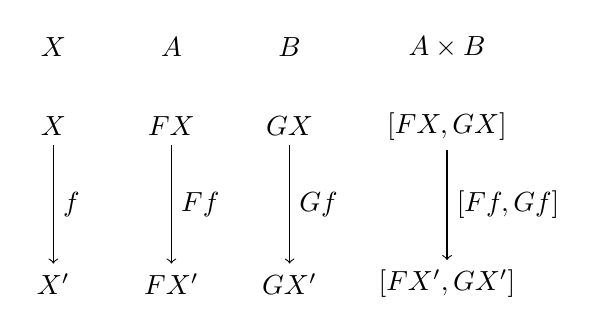
\begin{tikzpicture}[auto]
						\node (x) at (-1.5, 0) {$X$};
						\node (x') at (-1.5, -2) {$X'$};
						\node (a) at (0, 0) {$FX$};
						\node (a') at (0, -2) {$FX'$};
						\node (b) at (1.5, 0) {$GX$};
						\node (b') at (1.5, -2) {$GX'$};
						\node (ab) at (3.5, 0) {$[FX,GX]$};
						\node (ab') at (3.5, -2) {$[FX',GX']$};
						\draw[->] (x) to node{$f$}(x');
						\draw[->] (a) to node{$Ff$}(a');
						\draw[->] (b) to node{$Gf$}(b');
						\draw[->] (ab) to node{$[Ff,Gf]$}(ab');
						\node (cata) at (-1.5, 1) {$\cat{X}$};
						\node (cata) at (0, 1) {$\cat{A}$};
						\node (catb) at (1.5, 1) {$\cat{B}$};
						\node (catb) at (3.5, 1) {$\cat{A\times B}$};
					\end{tikzpicture}
				\end{center}
				\item[恒等射の保存]
				\begin{align*}
					\tuple{F,G}(id_X)&=\pcobj{F(id_X),G(id_X)}&\text{(射関数の定義)}\\
					&=\pcobj{id_{FX},id_{GX}}&\text{($F,G$の恒等射の保存)}\\
					&=id_{\pcobj{FX,GX}}&\text{(積圏の恒等射の定義)}
				\end{align*}
			よって恒等射を保つ
				\item[射の合成の保存]
				\begin{align*}
					\tuple{F,G}(f'\circ f)&=\pcobj{F(f'\circ f),G(f'\circ f)}&\text{(射関数の定義)}\\
					&=\pcobj{Ff'\circ Ff, Gf'\circ Gf}&\text{($F,G$の射の合成の保存)}\\
					&=\pcobj{Ff',Gf'}\circ\pcobj{Ff,Gf}&\text{(積圏の射の合成の定義)}\\
					&=\tuple{F,G}(f')\circ\tuple{F,G}(f)&\text{(射関数の定義)}
				\end{align*}
			よって射の合成を保つ。
			\end{mydescription}
		\end{quote}
	\end{define}
	\begin{prop}
		積圏$\cat{A\times B}$と射影関手$\Pi_\cat{A},\Pi_\cat{B}$の組$(\cat{A\times B},\Pi_\cat{A},\Pi_\cat{B})$は$\cat{Cat}$における積である。
	\end{prop}
	\begin{proof}
		積$(\cat{A\times B},\Pi_\cat{A},\Pi_\cat{B})$において、圏$\cat{X}$、関手$\functor{F}{X}{A}$、$\functor{G}{X}{B}$で構成される任意の組$(\cat{X},F,G)$に対して、$\Pi_\cat{A}\circ\tuple{F,G}=F,\ \Pi_\cat{B}\circ\tuple{F,G}=G$が成り立つような関手の対$\functor{\tuple{F,G}}{X}{A\times B}$が一意に存在することを示せばよい。
		\begin{center}
			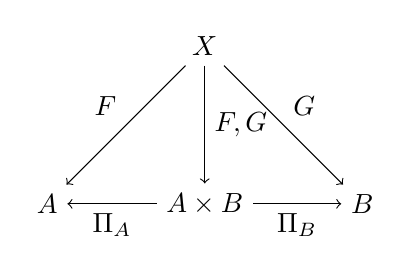
\begin{tikzpicture}[auto]
				\node (a) at (0, 0) {$\cat{A}$};
				\node (ab) at (2, 0) {$\cat{A\times B}$};
				\node (b) at (4, 0) {$\cat{B}$};
				\node (x) at (2, 2) {$\cat{X}$};
				\draw[->] (x) to node[swap]{$F$}(a);
				\draw[->] (x) to node{$G$}(b);
				\draw[->] (ab) to node{$\Pi_\cat{A}$}(a);
				\draw[->] (ab) to node[swap]{$\Pi_\cat{B}$}(b);
				\draw[->] (x) to node{$\tuple{F,G}$}(ab);
			\end{tikzpicture}
		\end{center}
		端的に述べるなら積圏、関手の対、射影関手の各々が持つ対象関数、射関数はそれぞれ積対象、射の対、射影射で構成されることから、積の普遍性を満たすことを示すのは難しくない。

		関手$F,G$の対象関数$F,G$、射影関手$\Pi_\cat{A},\Pi_\cat{B}$の対象関数$\pi_{\obj{A}},\pi_{\obj{B}}$、そして関手の対の対象関数$\tuple{F,G}$は、その定義により積の図式となる。
		すなわち対象関数$F,G$に対して対象関数$\tuple{F,G}$は一意に存在する。
		\begin{center}
			\begin{tikzpicture}[auto]
				\node (a) at (0, 0) {$\obj{A}$};
				\node (ab) at (4, 0) {$\obj{A}\times\obj{B}$};
				\node (abp) at (4, -1) {$\obj{A\times B}$};
				\node (b) at (8, 0) {$\obj{B}$};
				\node (x) at (4, 2) {$\obj{X}$};
				\draw[double distance=2pt] (ab) to (abp);
				\draw[->] (x) to node[swap]{$F$}(a);
				\draw[->] (x) to node{$G$}(b);
				\draw[->] (ab) to node{$\pi_{\obj{A}}$}(a);
				\draw[->] (ab) to node[swap]{$\pi_{\obj{B}}$}(b);
				\draw[->] (x) to node{$\tuple{F,G}$}(ab);
			\end{tikzpicture}
		\end{center}
		各射関数による積の図式は省略するが、同様に射関数$\tuple{F,G}$が一意に存在することが分かる。よって可換性を満たす対象関数と射関数も一意に存在することから、関手の対は積圏における射の対となり、$(\cat{A\times B},\Pi_\cat{A},\Pi_\cat{B})$は積の普遍性を満たす。
	\end{proof}
	\begin{define}[一点離散圏]
	一つの対象と一つの恒等射で構成される圏$\cat{1}$を\textbf{一点離散圏}とよぶ。
	\end{define}
	\begin{prop}[$\cat{Cat}$の終対象]
		$\cat{1}$は$\cat{Cat}$における終対象である。
	\end{prop}
	\begin{proof}
		任意の圏$\cat{C}$から一点離散圏$\cat{1}$への関手$!_{\cat{C}}$を考える。
		まず$\cat{1}$の対象$*$と射$id_*$は一つしか存在しない。そのため一点集合を$1$として
		\[\obj{1}=1,\ \arset{1}{*}{*}=1\]が成り立つ。

		よって対象関数$!_{\cat{C}}$は
		\begin{align*}
			&\mor{!_{\cat{C}}}{\obj{C}}{\obj{1}}\\
			=&\mor{!_{\cat{C}}}{\obj{C}}{1}
		\end{align*}
		となり一点集合への写像であることがわかる。よって任意の対象$A$に対して$!_{\cat{C}}(A)=*$が成り立ち、このような対象関数が一意に存在することが分かった。

		また任意の二対象$A,B$に対する射関数は
		\begin{align*}
			&\mor{{!_{\cat{C}}}_{A,B}}{\arset{C}{A}{B}}{\arset{1}{!_{\cat{C}}(A)}{!_{\cat{C}}(B)}}\\
			=&\mor{{!_{\cat{C}}}_{A,B}}{\arset{C}{A}{B}}{\arset{1}{*}{*}}\\
			=&\mor{{!_{\cat{C}}}_{A,B}}{\arset{C}{A}{B}}{1}\\
		\end{align*}と書ける。
		よって二対象$A,B$に対する各射関数も一意に存在することが分かった。

		関手$!_{\cat{C}}$の二つの写像が圏$\cat{C}$に対して一意に存在することわかる。
		よって任意の圏$\cat{C}$から一点離散圏$\cat{1}$への関手は一意に存在するから、一点離散圏$\cat{1}$は$\cat{Cat}$における終対象であることが示せた。
	\end{proof}
	\begin{prop}[対象と関手]
		任意の圏$\cat{C}$の元、つまり関手$\functor{A}{1}{C}$は圏$\cat{C}$の対象とみなせる。
	\end{prop}
	\begin{proof}
		関手$\functor{A}{1}{C}$は対象関数$\mor{F}{\obj{1}}{\obj{C}}$、射関数$\mor{F}{\arset{1}{*}{*}}{\arset{C}{F(*)}{F(*)}}$で構成される。このとき、$\obj{1}$は一点集合であるから、対象関数$F$は$\obj{C}$の元である。

		また射関数も同様に$\arset{C}{F(*)}{F(*)}$の元であるが、恒等射の保存より写される射は恒等射ただ一つであり、射関数は対象関数に対して一通りにしか定義できないから考慮しなくてもよい。

		よって関手$\functor{A}{1}{C}$は圏$\cat{C}$の対象とみなせる。
	\end{proof}
  集合の圏では$A\cong\arset{Set}{1}{A}$が成り立ったから、$\cat{Cat}$でも$\cat{A}\cong\arset{Cat}{\cat{1}}{\cat{A}}$のような主張が成り立つと考えるかもしれないが、$\arset{Cat}{\cat{1}}{\cat{A}}$はただの射集合、関手の集合であり、$\cat{Cat}$の対象にはならないから同型射となる関手を取ることができない。その上、この関手の集合は対象の集合であり圏の射の情報は全く含まれない。そのためこのような同型を考えるには$\cat{Cat}$における射集合的な圏を考える必要がある。この問題は後に関手圏と呼ばれる圏を定義することで解決する。

	関手としての対象の話に戻ると、積圏$\cat{A\times B}$の対象を$\pcobj{A,B}$と表したが、実際に対象$\functor{A}{1}{A}$と対象$\functor{B}{1}{B}$の関手の対$\functor{\tuple{A,B}}{1}{A\times B}$は$\cat{A\times B}$の対象になる。

	\subsection{特殊な関手}\label{chap-6.3-unique-functor}
  ある圏$\cat{C}$の二対象$A,B$の射集合$\arset{C}{A}{B}$は$A,B$で添字付けられていて、射写像$\arset{C}{A}{f}$も射で添字付けられているように見える。実際にこの操作は関手であるが、この段階ではこの操作を関手で表すことが難しい。そのため前提知識として双関手、反変関手を定義し見ていく。\\
	最初に対象や射を二つ取るような2変数関数のような関手、双関手について考える。
	\begin{define}[双関手]\label{def-bifunctor}
		積圏からの関手、つまり$\functor{F}{A\times B}{C}$となるような関手を\textbf{双関手}とする。

		また積圏の任意の対象$[A,B]$に対し、\[F(\pcobj{A,B})=F(A,B)\]と略記する。
		さらに積圏の射$\mor{\pcobj{f,id_B}}{\pcobj{A,B}}{\pcobj{A,B'}}$において\[F(\pcobj{f,id_B})=F(f,B)\]と表記する。
	\end{define}
	圏$\cat{A}$の射$f$と圏$\cat{B}$の射$g$がどのように圏$\cat{C}$に写されるのかを以下の可換図式で確認してほしい。等式としては示さないが、右の図式は関手の合成の保存によって可換になることに注意してほしい。
	\begin{center}
		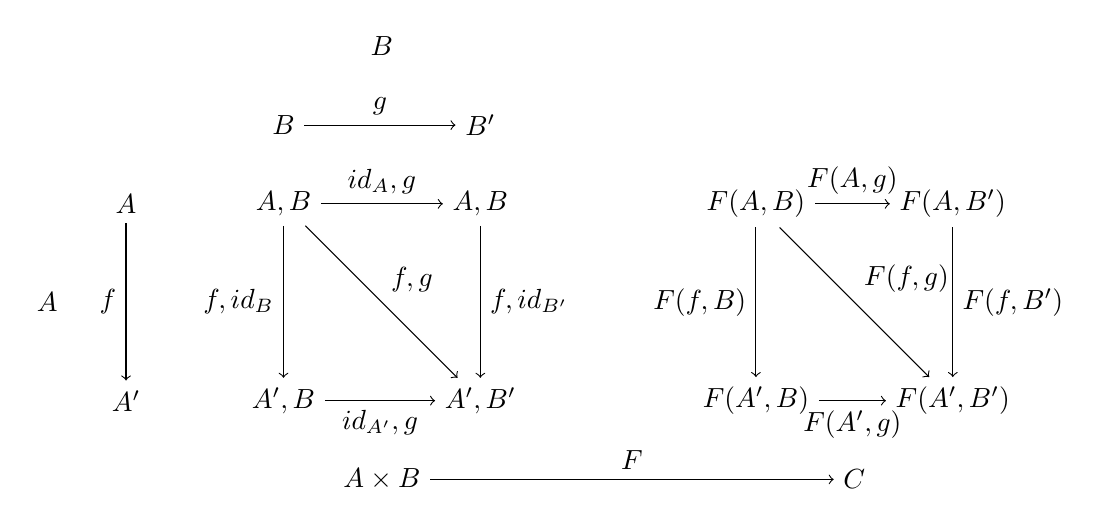
\begin{tikzpicture}[auto]
			\node (a) at (0, 0) {$A$};
			\node (a') at (0, -2.5) {$A'$};
			\node (b) at (2, 1) {$B$};
			\node (b') at (4.5, 1) {$B'$};
			\node (ab) at (2, 0) {$\pcobj{A,B}$};
			\node (a'b) at (2, -2.5) {$\pcobj{A',B}$};
			\node (ab') at (4.5, 0) {$\pcobj{A,B}$};
			\node (a'b') at (4.5, -2.5) {$\pcobj{A',B'}$};

			\node (fab) at (8, 0) {$F(A,B)$};
			\node (fa'b) at (8, -2.5) {$F(A',B)$};
			\node (fab') at (10.5, 0) {$F(A,B')$};
			\node (fa'b') at (10.5, -2.5) {$F(A',B')$};

			\node (cata) at (-1, -1.25) {$\cat{A}$};
			\node (catb) at (3.25, 2) {$\cat{B}$};
			\node (catab) at (3.25, -3.5) {$\cat{A\times B}$};
			\node (catc) at (9.25, -3.5) {$\cat{C}$};

			\draw[->] (a) to node[swap]{$f$}(a');
			\draw[->] (b) to node{$g$}(b');
			\draw[->] (ab) to node[swap]{$\pcobj{f,id_B}$}(a'b);
			\draw[->] (ab') to node{$\pcobj{f,id_{B'}}$}(a'b');
			\draw[->] (ab) to node{$\pcobj{id_A,g}$}(ab');
			\draw[->] (a'b) to node[swap]{$\pcobj{id_{A'},g}$}(a'b');
			\draw[->] (ab) to node{$\pcobj{f,g}$}(a'b');

			\draw[->] (fab) to node[swap]{$F(f,B)$}(fa'b);
			\draw[->] (fab') to node{$F(f,B')$}(fa'b');
			\draw[->] (fab) to node{$F(A,g)$}(fab');
			\draw[->] (fa'b) to node[swap]{$F(A',g)$}(fa'b');
			\draw[->] (fab) to node{$F(f,g)$}(fa'b');
			\draw[->] (catab) to node{$F$}(catc);
		\end{tikzpicture}
	\end{center}
  双関手は関手を量化とみなすのであれば、複数の圏のそれぞれの対象、射で同時に量化していると考えられる。\\
	次に双関手の例として積関手$\functor{-\times B}{C}{C}$を双関手に拡張しようと思う。
	\begin{define}[双積関手]\label{def-biproduct-functor}
		積を持つ圏$\cat{C}$上の\textbf{双積関手}$\functor{-\times -}{C\times C}{C}$を以下の写像で定義する。
		\begin{quote}
			\begin{mydescription}
				\item[対象関数] 対象関数を積圏$\cat{C\times C}$の任意の対象$\pcobj{A,B}$に対して\[(-\times -)(A,B)=A\times B\]と定義する。
				\item[射関数] 二対象$\pcobj{A,B},\pcobj{A',B'}$に対する射関数を任意の射$\mor{\pcobj{f,g}}{\pcobj{A,B}}{\pcobj{A',B'}}$に対して\[(-\times -)_{\pcobj{A,B},\pcobj{A',B'}}(f,g)=f\times g\]と定義する。
				\begin{center}
					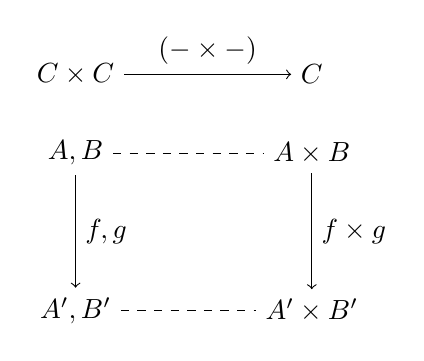
\begin{tikzpicture}[auto]
						\node (ab) at (0, 0) {$\pcobj{A,B}$};
						\node (a'b') at (0, -2) {$\pcobj{A',B'}$};
						\node (pab) at (3, 0) {$A\times B$};
						\node (pa'b') at (3, -2) {$A'\times B'$};
						\node (catcc) at (0, 1) {$\cat{C\times C}$};
						\node (catc) at (3, 1) {$\cat{C}$};
						\draw[-,dashed] (ab) to (pab);
						\draw[-,dashed] (a'b') to (pa'b');
						\draw[->] (ab) to node{$\pcobj{f,g}$}(a'b');
						\draw[->] (pab) to node{$f\times g$}(pa'b');
						\draw[->] (catcc) to node{$(-\times-)$}(catc);
					\end{tikzpicture}
				\end{center}

				\item[恒等射の保存] $(-\times -)(id_{\pcobj{A,B}})=id_{(-\times-)(A,B)}$を示せばよい。
				\begin{align*}
					(-\times -)(id_{\pcobj{A,B}})&=id_A\times id_B&\text{(射関数の定義)}\\
					&=\pcobj{id_A\circ\pi_A,id_B\circ\pi_B}&\text{(射の積の定義)}\\
					&=id_{A\times B}&\text{(射影射の対)}\\
					&=id_{(-\times-)(A,B)}&\text{(対象関数の定義)}
				\end{align*}
				よって恒等射を保つ。
				\item[射の合成の保存] $(-\times -)(f',g')\circ(-\times-)(f,g)=(-\times-)(\pcobj{f',g'}\circ\pcobj{f,g})$を示せばよい。
				\begin{align*}
					(-\times -)(f',g')\circ(-\times-)(f,g)&=(f'\times g')\circ(f\times g)&\text{(射関数の定義)}\\
					&=(f'\circ f)\times(g'\circ g)&\text{(積と合成の交換)}\\
					&=(-\times-)(f'\circ f,g'\circ g)&\text{(射関数の定義)}\\
					&=(-\times-)(\pcobj{f'\circ f,g'\circ g})\\
					&=(-\times-)(\pcobj{f',g'}\circ\pcobj{f,g})&\text{(積圏の射の合成の定義)}
				\end{align*}
				よって射の合成を保つ。
			\end{mydescription}
		\end{quote}
	\end{define}
	対象の積と圏の積が紛らわしいが、まず圏の積の対象$\pcobj{A,B}$は圏$\cat{C}$の$A$と$B$の積が存在しなくとも定義することができ、その点で対象の積$A\times B$より一般的な概念だと考えられる。よってイメージとしては圏$\cat{C}$の外側$\cat{C\times C}$で定義した対象の積もどき$[A,B]$を圏$\cat{C}$に積対象$A\times B$として挿入する操作が関手$(-\times-)$と考えられる。ただし、双積関手で写された対象が積の普遍性を満たすかどうかは現段階では説明できない。

	また以前に圏$\cat{C}$の射の積と積圏$\cat{C\times C}$の射の振る舞いが似ていることについて述べたが、実際に関手として二つの射の関係性を示すことができた。

  次に反変関手を定義するのであるが、これは厳密には関手ではない。しかし関手として扱う方法があり、そのために圏の双対について説明する。
	\begin{define}[双対圏]\label{def-opposite-category}
		ある圏$\cat{C}$に対する\textbf{双対圏}$\cat{C}^{op}$を以下の要素で定義する。
		\begin{quote}
			\begin{mydescription}
				\item[対象] $\obj{C^{op}}=\obj{C}$とする。

				また圏$\cat{C}$の対象$A$に対応する双対圏$\cat{C^{op}}$の対象も$A$であるが、$\cat{C^{op}}$の対象は$A^{op}$として表記上区別する。
				\item[射] 任意の二対象$A^{op}, B^{op}$に対して射集合を\[\arset{C^{op}}{B^{op}}{A^{op}}=\arset{C}{A}{B}\]と定義する。
				同様に射$\mor{f}{A}{B}$に対応する射を表記上$\mor{f^{op}}{B^{op}}{A^{op}}$とする。
				圏$\cat{C}$と双対圏$\cat{C^{op}}$では射の向きが入れ替わっていることに注意してほしい。
				\begin{center}
					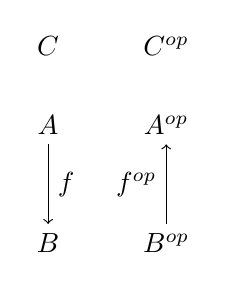
\begin{tikzpicture}[auto]
						\node (a) at (0, 0) {$A$};
						\node (b) at (0, -1.5) {$B$};
						\node (fa) at (1.5, 0) {$A^{op}$};
						\node (fb) at (1.5, -1.5) {$B^{op}$};
						\node (catc) at (0, 1) {$\cat{C}$};
						\node (catd) at (1.5, 1) {$\cat{C^{op}}$};
						\draw[->] (a) to node{$f$}(b);
						\draw[->] (fb) to node{$f^{op}$}(fa);
					\end{tikzpicture}
				\end{center}
				\item[射の合成] 圏$\cat{C}$の射$\mor{f}{A}{B}$、$\mor{g}{B}{C}$の合成射$\mor{g\circ f}{A}{C}$に対して、双対圏$\cat{C}^{op}$の射$\mor{f^{op}}{B^{op}}{A^{op}}$、$\mor{g^{op}}{C^{op}}{B^{op}}$の合成射を
				\[\mor{(g\circ f)^{op}=f^{op}\circ g^{op}}{C^{op}}{A^{op}}\]
				と定義する。
				圏$\cat{C}$と$\cat{C}^{op}$では射の合成の順序が入れ替わっていることに注意してほしい。
				\begin{center}
					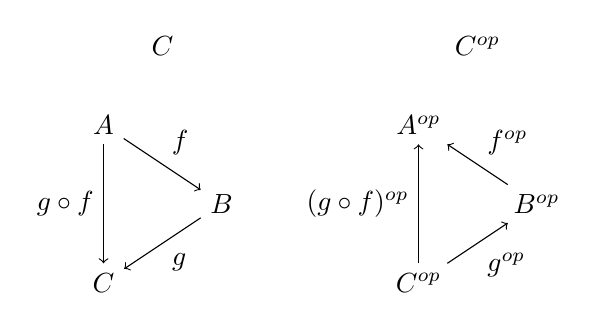
\begin{tikzpicture}[auto]
						\node (a) at (0, 0) {$A$};
						\node (b) at (1.5, -1) {$B$};
						\node (c) at (0, -2) {$C$};
						\node (fa) at (4, 0) {$A^{op}$};
						\node (fb) at (5.5, -1) {$B^{op}$};
						\node (fc) at (4, -2) {$C^{op}$};
						\node (catc) at (0.75, 1) {$\cat{C}$};
						\node (catd) at (4.75, 1) {$\cat{C^{op}}$};
						\draw[->] (a) to node{$f$}(b);
						\draw[->] (b) to node{$g$}(c);
						\draw[->] (a) to node[swap]{$g\circ f$}(c);
						\draw[->] (fb) to node[swap]{$f^{op}$}(fa);
						\draw[->] (fc) to node[swap]{$g^{op}$}(fb);
						\draw[->] (fc) to node{$(g\circ f)^{op}$}(fa);
					\end{tikzpicture}
				\end{center}
				\item[恒等射の存在]圏$\cat{C}$の任意の恒等射$\mor{id_A}{A}{A}$に対して、双対圏$\cat{C}^{op}$の恒等射を\[\mor{(id_A)^{op}=id_{A^{op}}}{A^{op}}{A^{op}}\]と定義する。
				\item[結合律] 合成可能な任意の射$f^{op},g^{op},h^{op}$において、
				\begin{align*}
					(f^{op}\circ g^{op})\circ h^{op}&=(g\circ f)^{op}\circ h^{op}\\
					&=(h\circ(g\circ f))^{op}\\
					&=((h\circ g)\circ f)^{op}\\
					&=f^{op}\circ (h\circ g)^{op}\\
					&=f^{op}\circ (g^{op}\circ h^{op})
				\end{align*}
				となるので結合律を満たす。
				\item[単位元律]任意の恒等射$id_{A^{op}}$、任意の射$\mor{f^{op}}{X^{op}}{A^{op}}$、$\mor{g^{op}}{A^{op}}{Y^{op}}$に対し$id_{A^{op}}\circ f^{op}=f^{op}$、$g^{op}\circ id_{A^{op}}=g^{op}$を示せばよい。
				\begin{align*}
					id_{A^{op}}\circ f^{op}&={id_A}^{op}\circ f^{op}&\text{(双対圏の恒等射の定義)}\\
					&=(f\circ id_A)^{op}&\text{(双対圏の射の合成の定義)}\\
					&=f^{op}&\text{(単位元律)}\\
					g^{op}\circ id_{A^{op}}&=g^{op}\circ {id_A}^{op}&\text{(双対圏の恒等射の定義)}\\
					&=(id_A\circ g)^{op}&\text{(双対圏の射の合成の定義)}\\
					&=g^{op}&\text{(単位元律)}\\
				\end{align*}
				よって単位元律を見たす。
			\end{mydescription}
		\end{quote}
	\end{define}
	圏の射をすべて反転した圏が双対圏であったが、圏から圏への関手から、双対圏から双対圏への関手を構成することができる。記述がややこしくなってしまったが、定義としては反転した射を反転した射に写すだけである。
	\begin{define}[双対関手]\label{def-opposite-functor}
		ある圏$\cat{C,D}$に対する双対圏$\cat{C}^{op},\cat{D}^{op}$と関手$\functor{F}{C}{D}$に対して、双対関手$\functor{F^{op}}{C^{op}}{D^{op}}$を以下の要素で定義する。
		\begin{quote}
			\begin{mydescription}
				\item[対象関数]対象関数$\mor{F^{op}}{C^{op}}{D^{op}}$を任意の対象$A^{op}$に対して
				\[F^{op}(A^{op})=(FA)^{op}\]と定義する。
				
				\item[射関数]対象関数と同様に、射関数\[\mor{{F^{op}}_{A^{op},B^{op}}}{\arset{C^{op}}{A^{op}}{B^{op}}}{\arset{D^{op}}{(FA)^{op}}{(FB)^{op}}}\]を任意の射$\mor{f}{A^{op}}{B^{op}}$に対して
				\[F^{op}(f^{op})=(Ff)^{op}\]と定義する。

				\begin{center}
					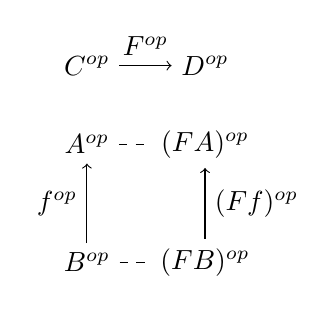
\begin{tikzpicture}[auto]
						\node (a) at (0, 0) {$A^{op}$};
						\node (b) at (0, -1.5) {$B^{op}$};
						\node (fa) at (1.5, 0) {$(FA)^{op}$};
						\node (fb) at (1.5, -1.5) {$(FB)^{op}$};
						\node (catc) at (0, 1) {$\cat{C^{op}}$};
						\node (catd) at (1.5, 1) {$\cat{D^{op}}$};
						\draw[-,dashed] (a) to (fa);
						\draw[-,dashed] (b) to (fb);
						\draw[->] (b) to node{$f^{op}$}(a);
						\draw[->] (fb) to node[swap]{$(Ff)^{op}$}(fa);
						\draw[->] (catc) to node{$F^{op}$}(catd);
					\end{tikzpicture}
					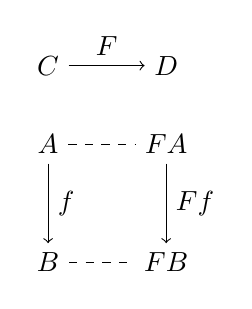
\begin{tikzpicture}[auto]
						\node (a) at (0, 0) {$A$};
						\node (b) at (0, -1.5) {$B$};
						\node (fa) at (1.5, 0) {$FA$};
						\node (fb) at (1.5, -1.5) {$FB$};
						\node (catc) at (0, 1) {$\cat{C}$};
						\node (catd) at (1.5, 1) {$\cat{D}$};
						\draw[-,dashed] (a) to (fa);
						\draw[-,dashed] (b) to (fb);
						\draw[->] (a) to node{$f$}(b);
						\draw[->] (fa) to node{$Ff$}(fb);
						\draw[->] (catc) to node{$F$}(catd);
					\end{tikzpicture}
				\end{center}
				\item[恒等射の保存]元の関手$F$の恒等射の保存に還元して$F^{op}(id_{A^{op}})=id_{(FA)^{op}}$を示す
				\begin{align*}
					F^{op}(id_{A^{op}})&=F^{op}(id_A)^{op}&\text{(双対圏の恒等射の定義)}\\
					&=(F(id_A))^{op}&\text{(双対関手の射関数の定義)}\\
					&=(id_{FA})^{op}&\text{($F$の恒等者の保存)}\\
					&=id_{(FA)^{op}}&\text{(双対圏の恒等射の定義)}
				\end{align*}
				
				\item[射の合成の保存]同様に元の関手の合成の保存に還元して\[F^{op}(f^{op}\circ g^{op})=F^{op}f^{op}\circ F^{op}g^{op}\]を示す。
				\begin{align*}
					F^{op}(f^{op}\circ g^{op})&= F^{op}(g\circ f)^{op}&\text{(双対圏の射の合成)}\\
					&=(F(g\circ f))^{op}&\text{(双対関手の射関数の定義)}\\
					&=(Fg\circ Ff)^{op}&\text{($F$の射の合成の保存)}\\
					&=(Fg)^{op}\circ (Ff)^{op}&\text{(双対圏の射の合成)}\\
					&=F^{op}f^{op}\circ F^{op}g^{op}&\text{(双対関手の射関数の定義)}
				\end{align*}
			\end{mydescription}
		\end{quote}
	\end{define}

	双対関手では反転した射を反転したまま写した。次に定義する反変関手では通常の射を反転した射に写すような捻れた操作を考える。この捻れによって関手の定義とは異なるものになることを注意してほしい。
	\begin{define}[反変関手]\label{def-contravariant-functor}
		圏$\cat{C}$から圏$\cat{D}$への\textbf{反変関手}と呼ばれる圏の間の写像$\functor{F}{C}{D}$を以下の写像と公理で定義する。
		\begin{quote}
			\begin{mydescription}
				\item[対象関数] $\cat{C}$の対象$A$に$\cat{D}$の対象$FA$を割り当てる対象関数\[\mor{F}{\obj{C}}{\obj{D}}\]を持つ必要がある。\\
				これは通常の関手と同じである。
				\item[射関数] $\cat{C}$の任意の各対象$A,B$において射$\mor{f}{A}{B}$に圏$\cat{D}$の射$\mor{Ff}{FB}{FA}$を割り当てる射関数\[\mor{F_{A,B}}{\arset{C}{A}{B}}{\arset{D}{FB}{FA}}\]を持つ必要がある。射の向きが変わってしまうが、関手と同様にこれも同様に対象$A,B$に対してそれぞれ存在する射関数$F_{A,B}$を総称して$F$と呼ぶことにする。
				\begin{center}
					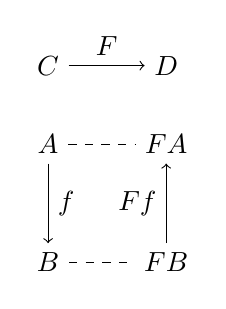
\begin{tikzpicture}[auto]
						\node (a) at (0, 0) {$A$};
						\node (b) at (0, -1.5) {$B$};
						\node (fa) at (1.5, 0) {$FA$};
						\node (fb) at (1.5, -1.5) {$FB$};
						\node (catc) at (0, 1) {$\cat{C}$};
						\node (catd) at (1.5, 1) {$\cat{D}$};
						\draw[-,dashed] (a) to (fa);
						\draw[-,dashed] (b) to (fb);
						\draw[->] (a) to node{$f$}(b);
						\draw[->] (fb) to node{$Ff$}(fa);
						\draw[->] (catc) to node{$F$}(catd);
					\end{tikzpicture}
				\end{center}
				双対圏を取る操作と同じように、射を写すときは射の向きを逆にする。
				\item[恒等射の保存] $F(id_A)=id_{FA}$が任意の恒等射で成り立つ。
				\item[射の合成の保存] 合成可能な任意の二射$f,g$において\[F(g\circ f)=Ff\circ Fg\]が成り立つ。

				\begin{center}
					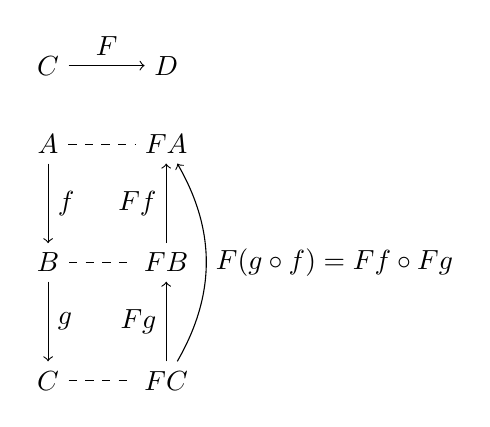
\begin{tikzpicture}[auto]
						\node (a) at (0, 0) {$A$};
						\node (b) at (0, -1.5) {$B$};
						\node (c) at (0, -3) {$C$};
						\node (fa) at (1.5, 0) {$FA$};
						\node (fb) at (1.5, -1.5) {$FB$};
						\node (fc) at (1.5, -3) {$FC$};
						\node (catc) at (0, 1) {$\cat{C}$};
						\node (catd) at (1.5, 1) {$\cat{D}$};
						\draw[-,dashed] (a) to (fa);
						\draw[-,dashed] (b) to (fb);
						\draw[-,dashed] (c) to (fc);
						\draw[->] (a) to node{$f$}(b);
						\draw[->] (b) to node{$g$}(c);
						\draw[->] (fb) to node{$Ff$}(fa);
						\draw[->] (fc) to node{$Fg$}(fb);
						\draw[->,bend right = 30] (fc) to node[swap]{$F(g\circ f)=Ff\circ Fg$}(fa);
						\draw[->] (catc) to node{$F$}(catd);
					\end{tikzpicture}
				\end{center}
				双対圏の射の合成と同じように、合成射を写すときは合成の順序を逆にして写す。
			\end{mydescription}
		\end{quote}
	\end{define}
	反変関手は関手とついているが、双対関手とは違い以前定義した関手の性質を満たさず、関手とはならない。そのため区別が必要な場合、一般の関手を\textbf{共変関手}と呼ぶことにする。\\
	また反変関手$\functor{F}{C}{D}$は双対圏によって共変関手$\functor{F}{C^{op}}{D}$とみなせることが図式から分かる。
		\begin{center}
			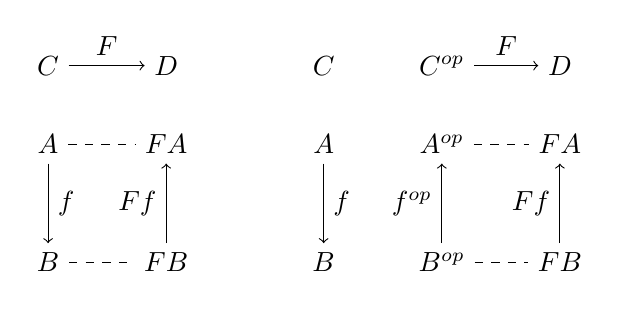
\begin{tikzpicture}[auto]
				\node (a) at (0, 0) {$A$};
				\node (b) at (0, -1.5) {$B$};
				\node (fa) at (1.5, 0) {$FA$};
				\node (fb) at (1.5, -1.5) {$FB$};
				\node (catc) at (0, 1) {$\cat{C}$};
				\node (catd) at (1.5, 1) {$\cat{D}$};
				\draw[-,dashed] (a) to (fa);
				\draw[-,dashed] (b) to (fb);
				\draw[->] (a) to node{$f$}(b);
				\draw[->] (fb) to node{$Ff$}(fa);
				\draw[->] (catc) to node{$F$}(catd);

				\node (a) at (3.5, 0) {$A$};
				\node (b) at (3.5, -1.5) {$B$};
				\node (aop) at (5, 0) {$A^{op}$};
				\node (bop) at (5, -1.5) {$B^{op}$};
				\node (fa) at (6.5, 0) {$FA$};
				\node (fb) at (6.5, -1.5) {$FB$};
				\node (catcop) at (3.5, 1) {$\cat{C}$};
				\node (catc) at (5, 1) {$\cat{C^{op}}$};
				\node (catd) at (6.5, 1) {$\cat{D}$};
				\draw[-,dashed] (aop) to (fa);
				\draw[-,dashed] (bop) to (fb);
				\draw[->] (bop) to node{$f^{op}$}(aop);
				\draw[->] (a) to node{$f$}(b);
				\draw[->] (fb) to node{$Ff$}(fa);
				\draw[->] (catc) to node{$F$}(catd);
			\end{tikzpicture}
		\end{center}
	
  \subsection{Hom関手}\label{chap-6.4-hom-functor}
  いよいよ射集合を取る操作が関手であることを示そう。その前に射写像を取る操作が関手の性質を満たすことを先に示しておく。
	\begin{prop}[共変射写像の恒等射の保存]\label{prop-preservation-identity-arrow-by-covariant-arrow-map}
		圏$\cat{C}$の任意の対象$X,A$において
		\[\arset{C}{X}{id_A}=id_{\arset{C}{X}{A}}\]が成り立つ。
		\begin{center}
			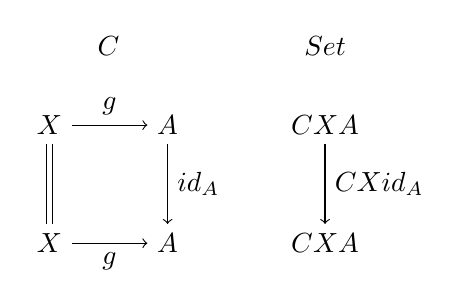
\begin{tikzpicture}[auto]
				\node (x) at (-1.5, 0) {$X$};
				\node (x2) at (-1.5, -1.5) {$X$};
				\node (a) at (0, 0) {$A$};
				\node (b) at (0, -1.5) {$A$};
				\node (ca) at (2, 0) {$\arset{C}{X}{A}$};
				\node (cb) at (2, -1.5) {$\arset{C}{X}{A}$};
				\node (catc) at (-0.75, 1) {$\cat{C}$};
				\node (catc) at (2, 1) {$\cat{Set}$};
				\draw[->] (ca) to node{$\arset{C}{X}{id_A}$}(cb);
				\draw[->] (a) to node{$id_A$}(b);
				\draw[double distance=2pt] (x) to (x2);
				\draw[->] (x) to node{$g$}(a);
				\draw[->] (x2) to node[swap]{$g$}(b);
			\end{tikzpicture}
		\end{center}
	\end{prop}
	\begin{proof}
		任意の射$\mor{g}{X}{A}$に対して
		\begin{align*}
			\arset{C}{X}{id_A}(g)&=id_A\circ g&\text{(共変射写像の定義)}\\
			&=g&\text{(単位元律)}\\
			&=id_{\arset{C}{X}{A}}(g)&\text{($\cat{Set}$の恒等射の定義)}\\
		\end{align*}
		よって$\arset{C}{X}{id_A}=id_{\arset{C}{X}{A}}$が成り立つ。
	\end{proof}
	\begin{prop}[共変射写像の合成の保存]\label{prop-preservation-composition-by-covariant-arrow-map}
		圏$\cat{C}$の任意の対象$X,A,B,C$と射$\mor{f}{A}{B}$、$\mor{g}{B}{C}$、$\mor{h}{X}{A}$に対して、
		\[\arset{C}{X}{g\circ f}=\arset{C}{X}{g}\circ\arset{C}{X}{f}\]が成り立つ。
		\begin{center}
			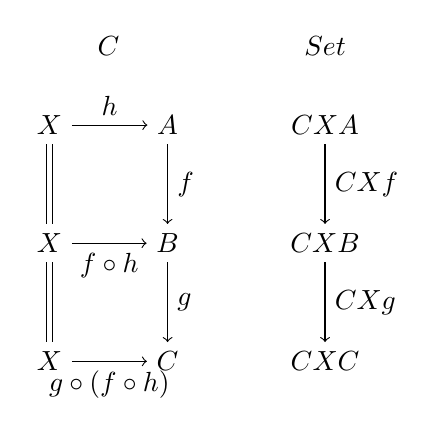
\begin{tikzpicture}[auto]
				\node (x) at (-1.5, 0) {$X$};
				\node (x2) at (-1.5, -1.5) {$X$};
				\node (x3) at (-1.5, -3) {$X$};
				\node (a) at (0, 0) {$A$};
				\node (b) at (0, -1.5) {$B$};
				\node (c) at (0, -3) {$C$};
				\node (ca) at (2, 0) {$\arset{C}{X}{A}$};
				\node (cb) at (2, -1.5) {$\arset{C}{X}{B}$};
				\node (cc) at (2, -3) {$\arset{C}{X}{C}$};
				\node (catc) at (-0.75, 1) {$\cat{C}$};
				\node (catc) at (2, 1) {$\cat{Set}$};
				\draw[->] (ca) to node{$\arset{C}{X}{f}$}(cb);
				\draw[->] (cb) to node{$\arset{C}{X}{g}$}(cc);
				\draw[->] (a) to node{$f$}(b);
				\draw[->] (b) to node{$g$}(c);
				\draw[double distance=2pt] (x) to (x2);
				\draw[double distance=2pt] (x2) to (x3);
				\draw[->] (x) to node{$h$}(a);
				\draw[->] (x2) to node[swap]{$f\circ h$}(b);
				\draw[->] (x3) to node[swap]{$g\circ(f\circ h)$}(c);
			\end{tikzpicture}
		\end{center}
	\end{prop}
	\begin{proof}
		任意の射$\mor{h}{X}{A}$に対して
		\begin{align*}
			\arset{C}{X}{g\circ f}(h)&=(g\circ f)\circ h&\text{(共変射関数の定義)}\\
			&=g\circ(f\circ h)&\text{(結合則)}\\
			&=\arset{C}{X}{g}(f\circ h)&\text{(共変射関数の定義)}\\
			&=\arset{C}{X}{g}(\arset{C}{X}{f}(h))&\text{(共変射関数の定義)}\\
			&=\arset{C}{X}{g}\circ\arset{C}{X}{f}(h)&\text{(写像の合成の定義)}\\
		\end{align*}
		よって$\arset{C}{X}{g\circ f}=\arset{C}{X}{g}\circ\arset{C}{X}{f}$が成り立つ。
	\end{proof}
	\begin{define}[共変Hom関手]\label{def-covariant-hom-functor}
		任意の圏$\cat{C}$とそのある対象$X$における共変Hom関手$\functor{\arset{C}{X}{-}}{C}{Set}$を以下の要素で定義する。
		\begin{quote}
			\begin{mydescription}
				\item[対象関数] 圏$\cat{C}$の任意の対象$A$に対して対象関数を
				\begin{align*}
					&\mor{\arset{C}{X}{-}}{\obj{C}}{\obj{Set}}\\
					&\arset{C}{X}{-}(A)=\arset{C}{X}{A}
				\end{align*}
				と定義する。
				\item[射関数] 圏$\cat{C}$の任意の対象$A,B$、射$\mor{f}{A}{B}$に対して射関数を
				\begin{align*}
					&\mor{\arset{C}{X}{-}_{A,B}}{\arset{C}{A}{B}}{\arset{Set}{\arset{C}{X}{A}}{\arset{C}{X}{B}}}\\
					&\arset{C}{X}{-}_{A,B}(f)=\arset{C}{X}{f}
				\end{align*}
				と定義する。
				\begin{center}
					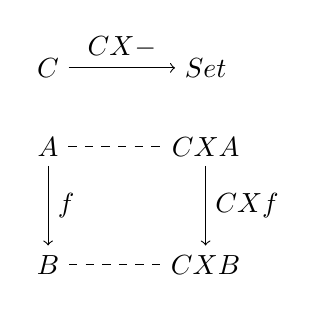
\begin{tikzpicture}[auto]
						\node (a) at (0, 0) {$A$};
						\node (b) at (0, -1.5) {$B$};
						\node (ca) at (2, 0) {$\arset{C}{X}{A}$};
						\node (cb) at (2, -1.5) {$\arset{C}{X}{B}$};
						\node (catc) at (0, 1) {$\cat{C}$};
						\node (catset) at (2, 1) {$\cat{Set}$};
						\draw[->] (ca) to node{$\arset{C}{X}{f}$}(cb);
						\draw[->] (a) to node{$f$}(b);
						\draw[->] (catc) to node{$\arset{C}{X}{-}$}(catset);
						\draw[-,dashed] (a) to (ca);
						\draw[-,dashed] (b) to (cb);
					\end{tikzpicture}
				\end{center}
				\item[恒等射の保存] 共変射写像の合成の保存より、$\arset{C}{X}{id_A}=id_{\arset{C}{X}{A}}$が成り立つ。
				\item[射の合成の保存] 共変射写像の恒等射の保存より、$\arset{C}{X}{g\circ f}=\arset{C}{X}{g}\circ\arset{C}{X}{f}$が成り立つ。
			\end{mydescription}
		\end{quote}
	\end{define}
	
	また反変射写像をとる操作を射関数とした関手は反変関手として定義する。
		\begin{define}[反変Hom関手]\label{def-contravariant-hom-functor}
		任意の圏$\cat{C}$とそのある対象$X$における反変Hom関手$\functor{\arset{C}{X}{-}}{C^{op}}{Set}$を以下の要素で定義する。
		\begin{quote}
			\begin{mydescription}
				\item[対象関数] 圏$\cat{C}$の任意の対象$A$に対して対象関数を
				\begin{align*}
					&\mor{\arset{C}{-}{X}}{\obj{C}}{\obj{Set}}\\
					&\arset{C}{-}{X}(A)=\arset{C}{X}{A}
				\end{align*}
				と定義する。
				\item[射関数] 圏$\cat{C}$の任意の対象$A,B$、射$\mor{f}{A}{B}$に対して射関数を
				\begin{align*}
					&\mor{\arset{C}{-}{X}_{A,B}}{\arset{C}{A}{B}}{\arset{Set}{\arset{C}{B}{X}}{\arset{C}{A}{X}}}\\
					&\arset{C}{-}{X}_{A,B}(f)=\arset{C}{f}{X}
				\end{align*}
				と定義する。
				\begin{center}
					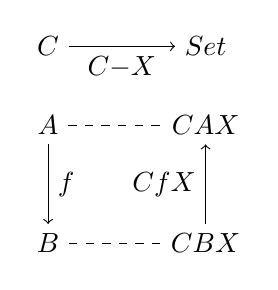
\begin{tikzpicture}[auto]
						\node (a) at (0, 0) {$A$};
						\node (b) at (0, -1.5) {$B$};
						\node (ca) at (2, 0) {$\arset{C}{A}{X}$};
						\node (cb) at (2, -1.5) {$\arset{C}{B}{X}$};
						\node (catc) at (0, 1) {$\cat{C}$};
						\node (catset) at (2, 1) {$\cat{Set}$};
						\draw[->] (cb) to node{$\arset{C}{f}{X}$}(ca);
						\draw[->] (a) to node{$f$}(b);
						\draw[->] (catc) to node[swap]{$\arset{C}{-}{X}$}(catset);
						\draw[-,dashed] (a) to (ca);
						\draw[-,dashed] (b) to (cb);
					\end{tikzpicture}
				\end{center}
				\item[恒等射の保存] 共変射写像の合成の保存と同様に$\arset{C}{id_A}{X}=id_{\arset{C}{A}{X}}$が成り立つ。
				\item[射の合成の保存] 共変射写像の恒等射の保存と同様に$\arset{C}{g\circ f}{X}=\arset{C}{f}{X}\circ\arset{C}{g}{X}$が成り立つ。
			\end{mydescription}
		\end{quote}
	\end{define}
  さて射集合、射写像を取る操作が関手であることを示せたから、これらが関手としてどのような性質をもつのか少し確認する。
	\begin{prop}[Hom関手の積の保存]\label{prop-preservation-product-by-hom-functor}
		圏$\cat{C}$の積$A\times B$に対して、\[\arset{C}{X}{A\times B}\cong \arset{C}{X}{A}\times \arset{C}{X}{B}\]が成り立つ。
	\end{prop}
	\begin{proof}
		$\arset{C}{X}{A}\times\arset{C}{X}{B}$は$\arset{C}{X}{A}$と$\arset{C}{X}{B}$の積であるが、$\arset{C}{X}{A\times B}$も同様に$\arset{C}{X}{A}$と$\arset{C}{X}{B}$の積であることを示せばよい。
		射影射をそれぞれ
		\begin{align*}
			&\pi_{\arset{C}{X}{A}}=\mor{\arset{C}{X}{\pi_A}}{\arset{C}{X}{A\times B}}{\arset{C}{X}{A}}\\
			&\pi_{\arset{C}{X}{B}}=\mor{\arset{C}{X}{\pi_B}}{\arset{C}{X}{A\times B}}{\arset{C}{X}{B}}
		\end{align*}
		として、組$(\arset{C}{X}{A\times B},\arset{C}{X}{\pi_A},\arset{C}{X}{\pi_B})$が積の普遍性を満たすことを証明する。つまり$\cat{Set}$の任意の対象$Y$と任意の二射$\mor{i}{Y}{\arset{C}{X}{A}}$、$\mor{j}{Y}{\arset{C}{X}{B}}$に対して、
		\begin{align*}
			&\arset{C}{X}{\pi_A}\circ\tuple{i,j}=i\\
			&\arset{C}{X}{\pi_B}\circ\tuple{i,j}=j
		\end{align*}
		が成り立つような射$\mor{\tuple{i,j}}{Y}{\arset{C}{X}{A\times B}}$が一意に存在することを示せばよい。\\
    証明の方向性としては集合の圏$\cat{Set}$の射\[\mor{i}{Y}{\arset{C}{X}{A}},\ \mor{j}{Y}{\arset{C}{X}{A}}\]に$Y$の元$y$を適用すると、圏$\cat{C}$の射\[\mor{i(y)}{X}{A},\ \mor{j(y)}{X}{B}\]が得られるが、集合の圏$\cat{Set}$の射の対$\tuple{i,j}$の存在と一意性を、圏$\cat{C}$の積の普遍性で示すことで証明する。\\
		まずは図式を可換にする$\tuple{i,j}$を定義し、常に存在することを示す。
		\begin{center}
			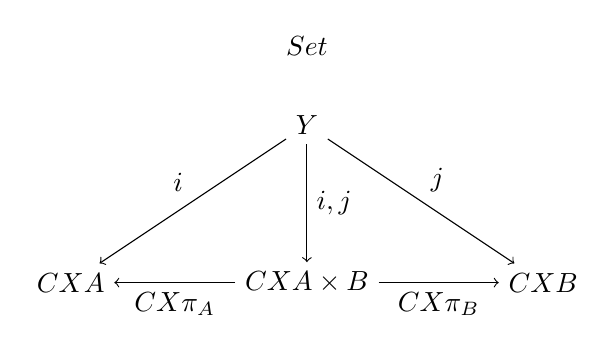
\begin{tikzpicture}[auto]
				\node (set) at (3, 3) {$\cat{Set}$};
				\node (xa) at (0, 0) {$\arset{C}{X}{A}$};
				\node (xab) at (3, 0) {$\arset{C}{X}{A\times B}$};
				\node (xb) at (6, 0) {$\arset{C}{X}{B}$};
				\node (y) at (3, 2) {$Y$};
				\draw[->] (xab) to node{$\arset{C}{X}{\pi_A}$}(xa);
				\draw[->] (xab) to node[swap]{$\arset{C}{X}{\pi_B}$}(xb);
				\draw[->] (y) to node[swap]{$i$}(xa);
				\draw[->] (y) to node{$j$}(xb);
				\draw[->] (y) to node{$\tuple{i,j}$}(xab);
			\end{tikzpicture}
		\end{center}
		ここで対象$Y$の任意の元$y$を取り適用すると、圏$\cat{C}$の射$\mor{i(y)}{X}{A}$、$\mor{j(y)}{X}{B}$が得られる。

		射$i,j$は$\cat{Set}$の射であるが、値を適用した$i(y),j(y)$もまた$\cat{C}$の射であることに注意してほしい。もし圏$\cat{C}$で対象$X$の元$x$が取れるなら、さらに値を適用して対象$A$の元$i(y)(x)$が取れる。

		圏$\cat{C}$の積$(A\times B,\pi_A,\pi_B)$に対して射$i(y),j(y)$の射の対\[\mor{\tuple{i(y),j(y)}}{X}{A\times B}\]を考える。
		\begin{center}
			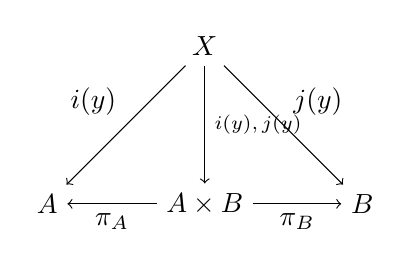
\begin{tikzpicture}[auto]
				\node (a) at (0, 0) {$A$};
				\node (b) at (4, 0) {$B$};
				\node (ab) at (2, 0) {$A\times B$};
				\node (x) at (2, 2) {$X$};
				\draw[->] (ab) to node {$\pi_A$}(a);
				\draw[->] (ab) to node[swap] {$\pi_B$}(b);
				\draw[->] (x) to node[swap] {$i(y)$}(a);
				\draw[->] (x) to node {$j(y)$}(b);
				\draw[->] (x) to node {\scriptsize{$\tuple{i(y),j(y)}$}}(ab);
			\end{tikzpicture}
		\end{center}
		このような射の対は任意の射$i(y),j(y)$に対して存在するから、任意の$y$に対しても存在する。
		よって$\cat{Set}$の射の対$\tuple{i,j}$を任意の$y$に対して\[\tuple{i,j}(y)=\tuple{i(y),j(y)}\]と定義できた。
		次に$\tuple{i,j}$が図式を可換にすることを示す。

		同様に$Y$の任意の元$y$に対し
		\begin{align*}
			\arset{C}{X}{\pi_A}\circ\tuple{i,j}(y)&=\arset{C}{X}{\pi_A}(\tuple{i,j}(y))&\text{(射の合成の定義)}\\
			&=\arset{C}{X}{\pi_A}(\tuple{i(y),j(y)})&\text{($\tuple{i,j}$の定義)}\\
			&=\pi_A\circ(\tuple{i(y),j(y)})&\text{(共変射写像の定義)}\\
			&=i(y)&\text{(射の対の可換性)}
		\end{align*}
		よって$\arset{C}{X}{\pi_A}\circ\tuple{i,j}=i$が成り立つ。同様に$\arset{C}{X}{\pi_B}\circ\tuple{i,j}=j$も成り立つ。

		次に射の対$\tuple{i,j}$の一意性を示す。
		ある射$\mor{k}{Y}{\arset{C}{X}{A\times B}}$が
		\begin{align*}
			&\arset{C}{X}{\pi_A}\circ k=i\\
			&\arset{C}{X}{\pi_B}\circ k=j
		\end{align*}
		を満たすとき、$h=\tuple{i,j}$が成り立つことを示せばよい。

		$Y$の任意の元$y$に対し
		\begin{align*}
			i(y)&=(\arset{C}{X}{\pi_A}\circ k)(y)\\
			&=\arset{C}{X}{\pi_A}(k(y))&\text{(射の合成の定義)}\\
			&=\pi_A\circ(k(y))&\text{(共変射写像の定義)}
		\end{align*}
		よって$\pi_A\circ(k(y))=i(y)$が成り立つ。同様に$\pi_A\circ(k(y))=i(y)$も成り立つ。
		すると$\cat{C}$の積$A\times B$の射の対$\tuple{i,j}(y)$の一意性より、$k(y)=\tuple{i,j}(y)$となる。
		これは任意の$y$で成り立つから$k=\tuple{i,j}$となり、$\tuple{i,j}$は$i,j$に対して一意に存在することが示せた。
		\begin{center}
			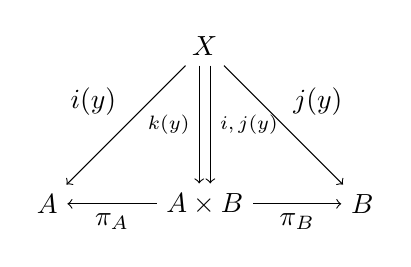
\begin{tikzpicture}[auto]
				\node (a) at (0, 0) {$A$};
				\node (b) at (4, 0) {$B$};
				\node (ab) at (2, 0) {$A\times B$};
				\node (x) at (2, 2) {$X$};
				\draw[->] (ab) to node {$\pi_A$}(a);
				\draw[->] (ab) to node[swap] {$\pi_B$}(b);
				\draw[->] (x) to node[swap] {$i(y)$}(a);
				\draw[->] (x) to node {$j(y)$}(b);
				\draw[->,transform canvas={xshift=+2pt}] (x) to node {\scriptsize{$\tuple{i,j}(y)$}}(ab);
				\draw[->,transform canvas={xshift=-2pt}] (x) to node[swap] {\scriptsize{$k(y)$}}(ab);
			\end{tikzpicture}
		\end{center}
		よって組$(\arset{C}{X}{A\times B},\arset{C}{X}{\pi_A},\arset{C}{X}{\pi_B})$は積の普遍性を満たす。つまり$\arset{C}{X}{A\times B}$は$\arset{C}{X}{A}$と$\arset{C}{X}{B}$の積であり、積の一意性より、\[\arset{C}{X}{A\times B}\cong \arset{C}{X}{A}\times \arset{C}{X}{B}\]が成り立つ。
	\end{proof}
	かなり長い証明になってしまったが、$\arset{C}{X}{A\times B}\cong \arset{C}{X}{A}\times \arset{C}{X}{B}$を示すだけなら同型射となるような射を定義して同型射であることを証明すればよい。こちらの方が簡単ではあるが、同型射を射集合を用いた議論に慣れてもらうためこのように証明した。

	さてこの同型の意味を考えると、任意の二射$\mor{f}{X}{A}$、$\mor{g}{X}{B}$と射の対$\mor{\tuple{f,g}}{X}{A\times B}$が一対一対応をする、ということになる。ただし現段階では逆は成り立たない。

  また、証明中では特に区別しなかったが、集合の圏の積による射の対を$\mor{[f,g]}{1}{\arset{C}{X}{A}\times\arset{C}{X}{B}}$、圏$\cat{C}$の積による射の対を$\mor{\tuple{f,g}}{X}{A\times B}$として、同型射をそれぞれ、\[\mor{i}{\arset{C}{X}{A\times B}}{\arset{C}{X}{A}\times\arset{C}{X}{B}}\]\[\mor{i^{-1}}{\arset{C}{X}{A}\times\arset{C}{X}{B}}{\arset{C}{X}{A\times B}}\]とすると、\[i(\tuple{f,g})=[f,g],\ i^{-1}([f,g])=\tuple{f,g}\]となる射であることが、積の一意性の証明から分かる。
  つまり、これらの同型射は、圏$\cat{C}$の射の対と集合の圏の射の対を相互に変換する写像であることが分かる。


  これらの射が既存の射を用いてどのように構成されるかを示したいところではあるが、射の対の種類が更に増えてややこしくなってしまうため、ここでは結果だけを示した。

	次に自明ではあるが、共変Hom関手が終対象を保つことを同様に証明する。
	\begin{prop}[Hom関手の終対象の保存]\label{prop-preservation-terminal-object-by-hom-functor}
		圏$\cat{C}$の終対象$1$と圏$\cat{Set}$の任意の対象$X$と終対象$I$に対して\[\arset{C}{X}{1}\cong I\]が成り立つ。
	\end{prop}
	\begin{proof}
		$\arset{C}{X}{1}$が$\cat{Set}$における終対象であることを示せばよい。つまり$\cat{Set}$の任意の対象$Y$に対して\[\mor{!_Y}{Y}{\arset{C}{X}{1}}\]が一意に存在することを証明する。

		射$\mor{!_Y}{Y}{\arset{C}{X}{1}}$が少なくとも一つは存在すると仮定する。
		対象$Y$の任意の元$y$を$!_Y$に適用すると圏$\cat{C}$の射$\mor{!_Y(y)}{X}{1}$が得られるが、終対象$1$の普遍性よりこのような射は少なくとも一つは存在する。よって任意の$y$において$!_Y(y)$が存在するから、実際に射$!_Y$は存在する。
		\begin{center}
			\begin{tikzpicture}[auto]
				\node (set) at (1, 1) {$\cat{Set}$};
				\node (1) at (0, 0) {$Y$};
				\node (1') at (2, 0) {$\arset{C}{X}{1}$};
				\node (set) at (5, 1) {$\cat{C}$};
				\node (x) at (4, 0) {$X$};
				\node (t) at (6, 0) {$1$};
				\draw[->] (1) to node{$!_Y$}(1');
				\draw[->] (x) to node{$!_Y(y)$}(t);
			\end{tikzpicture}
		\end{center}
		次に$\mor{!_Y}{Y}{\arset{C}{X}{1}}$の一意性を示す。つまり射$\mor{h}{Y}{\arset{C}{X}{1}}$が存在したとき、$!_Y=h$が成り立てばよい。

		対象$Y$の任意の元$y$において射$\mor{h(y)}{X}{1}$に対して圏$\cat{C}$の終対象の普遍性より、$\mor{!_Y(y)}{X}{1}$なる射は一意に存在する。よって$!_Y(y)=h(y)$となり、任意の元$y$で成り立つから$!_Y=h$となる。

		\begin{center}
			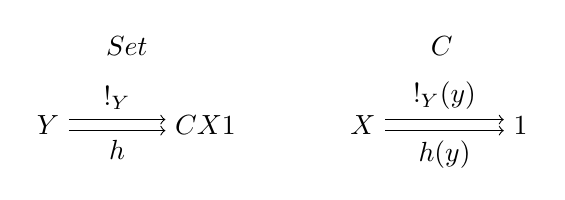
\begin{tikzpicture}[auto]
				\node (set) at (1, 1) {$\cat{Set}$};
				\node (1) at (0, 0) {$Y$};
				\node (1') at (2, 0) {$\arset{C}{X}{1}$};
				\node (set) at (5, 1) {$\cat{C}$};
				\node (x) at (4, 0) {$X$};
				\node (t) at (6, 0) {$1$};
				\draw[->,transform canvas={yshift=2pt}] (1) to node{$!_Y$}(1');
				\draw[->,transform canvas={yshift=2pt}] (x) to node{$!_Y(y)$}(t);
				\draw[->,transform canvas={yshift=-2pt}] (1) to node[swap]{$h$}(1');
				\draw[->,transform canvas={yshift=-2pt}] (x) to node[swap]{$h(y)$}(t);
			\end{tikzpicture}
		\end{center}
		$\mor{!_Y}{Y}{\arset{C}{X}{1}}$なる射が一意に存在することが示せたから、$\arset{C}{X}{1}$は$\cat{Set}$における終対象となる。よって終対象の一意性より、\[\arset{C}{X}{1}\cong I\]が成り立つ。
	\end{proof}

	次に積関手を双積関手に一般化したように、共変Hom関手、反変Hom関手を双関手として定義する。
	\begin{define}[双Hom関手]\label{def-dihom-functor}
		任意の圏$\cat{C}$における\textbf{双Hom関手}$\functor{C(-,-)}{C^{op}\times C}{Set}$を以下の要素で定義する。
		\begin{quote}
			\begin{mydescription}
				\item[対象関数] 積圏$\cat{C^{op}\times C}$の任意の対象$[A,B]$に対して対象関数を
				\begin{align*}
					&\mor{\arset{C}{-}{-}}{\obj{C^{op}\times C}}{\obj{Set}}\\
					&\arset{C}{-}{-}([A,B])=\arset{C}{A}{B}
				\end{align*}
				と定義する。
				\item[射関数]射関数を定義する前に共変射写像、反変射写像の双Hom関手版を定義する。
				圏$\cat{C^{op}}$の任意の射$\mor{f^{op}}{A^{op}}{A'^{op}}$、つまり圏$\cat{C}$の射$\mor{f}{A'}{A}$と圏$\cat{C}$の任意の射$\mor{g}{B}{B'}$に対し射写像\[\mor{\arset{C}{f}{g}}{\arset{C}{A}{B}}{\arset{C}{A'}{B'}}\]を任意の射$\mor{h}{A}{B}$において、
				\begin{align*}
					\arset{C}{f}{g}&=\arset{C}{f}{B'}\circ\arset{C}{A}{g}\\
					&=\arset{C}{A'}{g}\circ\arset{C}{f}{B}\\
					\arset{C}{f}{g}(h)&=g\circ h\circ f\\
				\end{align*}
				と定義する。

				\begin{center}
					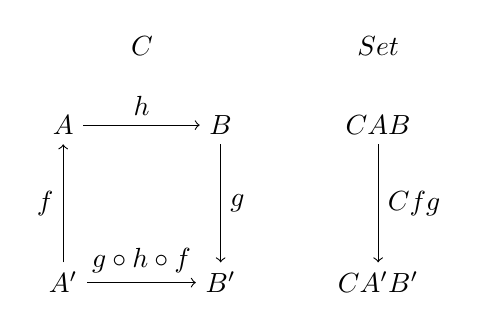
\begin{tikzpicture}[auto]
						\node (A) at (0, 0) {$A$};
						\node (A') at (0, -2) {$A'$};
						\node (B) at (2, 0) {$B$};
						\node (B') at (2, -2) {$B'$};
						\draw[->] (A') to node{$f$}(A);
						\draw[->] (B) to node{$g$}(B');
						\draw[->] (A) to node{$h$}(B);
						\draw[->] (A') to node{$g\circ h\circ f$}(B');
						\node (AB) at (4, 0) {$\arset{C}{A}{B}$};
						\node (A'B') at (4, -2) {$\arset{C}{A'}{B'}$};
						\draw[->] (AB) to node{$\arset{C}{f}{g}$}(A'B');
						\node (catc) at (1, 1) {$\cat{C}$};
						\node (catset) at (4, 1) {$\cat{Set}$};
					\end{tikzpicture}
				\end{center}

				圏$\cat{C^{op}\times C}$の任意の対象$[A,B],[A',B']$、射$\mor{f}{A}{B}$に対して射関数を
				\begin{align*}
					&\mor{\arset{C}{-}{-}}{\arset{(C^{op}\times C)}{[A,B]}{[A',B']}}{\arset{Set}{\arset{C}{A}{B}}{\arset{C}{A'}{B'}}}\\
					&\arset{C}{-}{-}([f,g])=\arset{C}{f}{g}
				\end{align*}
				と定義する。
				\begin{center}
					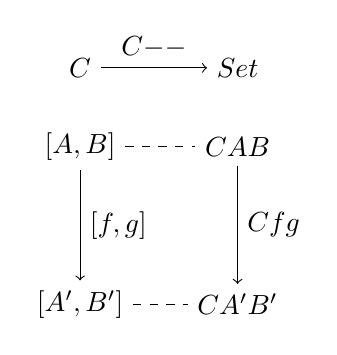
\begin{tikzpicture}[auto]
						\node (ab) at (0, 0) {$[A,B]$};
						\node (a'b') at (0, -2) {$[A',B']$};
						\draw[->] (ab) to node{$[f,g]$}(a'b');
						\node (sab) at (2, 0) {$\arset{C}{A}{B}$};
						\node (sa'b') at (2, -2) {$\arset{C}{A'}{B'}$};
						\draw[->] (sab) to node{$\arset{C}{f}{g}$}(sa'b');
						\draw[-,dashed] (ab) to (sab);
						\draw[-,dashed] (a'b') to (sa'b');
						\node (catc) at (0, 1) {$\cat{C}$};
						\node (catset) at (2, 1) {$\cat{Set}$};
						\draw[->] (catc) to node{$\arset{C}{-}{-}$}(catset);
					\end{tikzpicture}
				\end{center}
				\item[恒等射の保存] 圏$\cat{C^{op}\times C}$の任意の対象$[A,B]$に対して\[\arset{C}{-}{-}(id_{[A,B]})=\mor{id_{\arset{C}{-}{-}([A,B])}}{\arset{C}{A}{B}}{\arset{C}{A}{B}}\]を示せばよい。

				任意の積圏の射$\mor{f}{A}{B}$に対して
				\begin{align*}
					\arset{C}{-}{-}(id_{[A,B]})(f)&=\arset{C}{-}{-}([id_A,id_B])(f)&\text{(積圏の恒等射の定義)}\\
					&=\arset{C}{id_A}{id_B}(f)&\text{(対象関数の定義)}\\
					&=id_B\circ f\circ id_A&\text{(射写像の定義)}\\
					&=f&\text{(圏$\cat{C}$の単位元律)}\\
					&=id_{\arset{C}{A}{B}}(f)&\text{($\cat{Set}$の単位元律)}\\
					&=id_{\arset{C}{-}{-}([A,B])}(f)&\text{(対象関数の定義)}
				\end{align*}
				よって$\arset{C}{-}{-}(id_{[A,B]})=id_{\arset{C}{-}{-}([A,B])}$が成り立ち恒等射の保存が成り立つ。


				\item[射の合成の保存] $\cat{Set}$の任意の射写像$\mor{\arset{C}{f}{g}}{\arset{C}{A}{B}}{\arset{C}{A'}{B'}}$、$\mor{\arset{C}{f'}{g'}}{\arset{C}{A'}{B'}}{\arset{C}{A''}{B''}}$に対して\[\arset{C}{f'}{g'}\circ\arset{C}{f}{g}=\arset{C}{f\circ f'}{g'\circ g}\]が成り立てばよい。

				圏$\cat{C}$の任意の射$\mor{h}{A}{B}$に対して
				\begin{align*}
					(\arset{C}{f'}{g'}\circ\arset{C}{f}{g})(h)&=(\arset{C}{f'}{g'})(g\circ h\circ f)&\text{(射写像の定義)}\\
					&=g'\circ(g\circ h\circ f)\circ f'&\text{(射写像の定義)}\\
					&=(g'\circ g)\circ h\circ(f\circ f')&\text{(結合律)}\\
					&=\arset{C}{f\circ f'}{g'\circ g}(h)&\text{(射写像の定義)}\\
				\end{align*}
				よって$\arset{C}{f'}{g'}\circ\arset{C}{f}{g}=\arset{C}{f\circ f'}{g'\circ g}$となり射の合成の保存が成り立つ。
			\end{mydescription}
		\end{quote}
	\end{define}

	双積関手、双Hom関手を定義したときは完全に新しい関手として対象関数、射関数から定義した。しかし、これらの例のように、右側と左側の関手がそれぞれ定まっていて、ある条件を満たしていれば二つの関手から双関手を定義できる。\\メリットとしてこの定義を用いれば双関手の恒等射の保存と合成の保存を個別に証明しなくても済む。
	\begin{define}[二つの関手による双関手の定義]\label{def-bifunctor-by-two-functors}
		圏$\cat{B}$の任意の対象$B$に対して定義される関手$\functor{F_B}{A}{C}$と、圏$\cat{A}$の任意の対象$A$に対して定義される関手$\functor{G_A}{B}{C}$が存在し、任意の二対象$A,B$に対して\[{F_B}A={G_A}B\]が成り立ち、	任意の二射$\mor{f}{A}{A'}$、$\mor{g}{B}{B'}$に対して\[{G_{A'}}g\circ {F_B}f = {F_{B'}}f\circ {G_A}g\]が成り立つとする。
		\begin{center}
			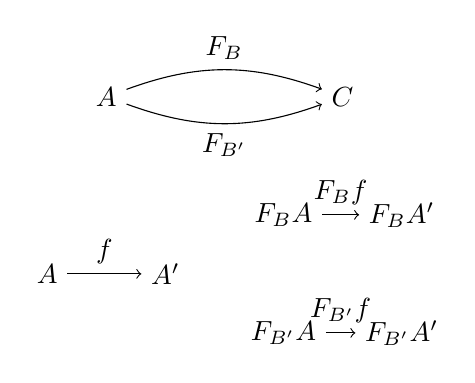
\begin{tikzpicture}[auto]
				\node (A) at (0, 0.75) {$A$};
				\node (B) at (1.5, 0.75) {$A'$};
				\node (FA) at (3, 1.5) {${F_B}A$};
				\node (FB) at (4.5, 1.5) {${F_B}A'$};
				\node (GA) at (3, 0) {${F_{B'}}A$};
				\node (GB) at (4.5, 0) {${F_{B'}}A'$};

				\node (catc) at (0.75, 3) {$\cat{A}$};
				\node (catd) at (3.75, 3) {$\cat{C}$};

				\draw[->] (A) to node{$f$}(B);
				\draw[->] (FA) to node{${F_B}f$}(FB);
				\draw[->] (GA) to node{${F_{B'}}f$}(GB);
				\draw[->,bend left = 20] (catc) to node (funcf){$F_B$}(catd);
				\draw[->,bend right = 20] (catc) to node (funcg)[swap]{$F_{B'}$}(catd);
			\end{tikzpicture}
			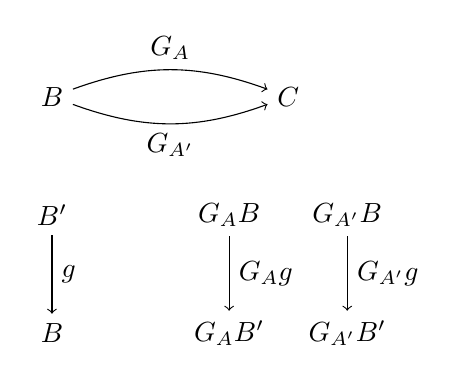
\begin{tikzpicture}[auto]
				\node (A) at (0.75, 0) {$B$};
				\node (B) at (0.75, 1.5) {$B'$};
				\node (FA) at (3, 1.5) {${G_A}B$};
				\node (FB) at (4.5, 1.5) {${G_{A'}}B$};
				\node (GA) at (3, 0) {${G_{A}}B'$};
				\node (GB) at (4.5, 0) {${G_{A'}}B'$};

				\node (catc) at (0.75, 3) {$\cat{B}$};
				\node (catd) at (3.75, 3) {$\cat{C}$};

				\draw[->] (B) to node{$g$}(A);
				\draw[->] (FA) to node{${G_A}g$}(GA);
				\draw[->] (FB) to node{${G_{A'}}g$}(GB);

				\draw[->,bend left = 20] (catc) to node (funcf){$G_A$}(catd);
				\draw[->,bend right = 20] (catc) to node (funcg)[swap]{$G_{A'}$}(catd);
			\end{tikzpicture}
		\end{center}


		この時、双関手$\functor{H}{A\times B}{C}$を
		\begin{quote}
			\begin{mydescription}
				\item[対象関数] 対象関数\[\mor{H}{\obj{A\times B}}{\obj{C}}\]を積圏の任意の対象$\pcobj{A,B}$に対して
				\[H(A,B)={F_B}A={G_A}B\]と定義する。
				\item[射関数]射関数\[\mor{H_{\pcobj{A,A'},\pcobj{B,B'}}}{\arset{A\times B}{\pcobj{A,B}}{\pcobj{A',B'}}}{\arset{C}{H(A,B)}{H(A',B')}}\]を積圏の任意の射\[\mor{\pcobj{f,g}}{\pcobj{A,B}}{\pcobj{A',B'}}\]に対して、\[H_{\pcobj{A,A'},\pcobj{B,B'}}(\pcobj{f,g})={G_{A'}}g\circ {F_B}f = {F_{B'}}f\circ {G_A}g\]と定義する。
				\item[恒等射の保存]$H(id_{\pcobj{A,B}})=id_{H(A,B)}$を示せばよい。
				\begin{align*}
					H(id_{\pcobj{A,B}})&=H(id_A,id_B)&\text{(積圏の恒等射の定義)}\\
					&=G_A(id_B)\circ F_B(id_A)&\text{(双関手の射関数)}\\
					&=id_{H(A,B)}\circ id_{H(A,B)}&\text{(関手の恒等射の保存)}\\
					&=id_{H(A,B)}&\text{(積圏の単位減律)}
				\end{align*}
				よって恒等射を保存する。
				\item[射の合成の保存]$H(f',g')\circ H(f,g)=H(f'\circ f,g'\circ g)$を示せばよい。
				\begin{align*}
					H(f',g')\circ H(f,g)&=(G_{A''}g'\circ F_{B'}f')\circ(G_{A'}\circ F_Bf)&\text{(射関数の定義)}\\
					&=G_{A''}g'\circ (F_{B'}f'\circ G_{A'})\circ  F_Bf&\text{(積圏の結合律)}\\
					&=G_{A''}g'\circ G_{A''}g\circ F_Bf'\circ  F_Bf&\text{(射関数の定義)}\\
					&=(G_{A''}g'\circ G_{A''}g)\circ (F_Bf'\circ  F_Bf)&\text{(積圏の結合則)}\\
					&=G_{A''}(g'\circ g)\circ F_B(f'\circ f)&\text{($G_{A''}$と$F_B$の合成の保存)}\\
					&=H(f'\circ f,g'\circ g)&\text{(射関数の定義)}\\
				\end{align*}
			\end{mydescription}
		\end{quote}
		証明が少し複雑になってしまったが、何とか証明できた。
	\end{define}
	次に例として二つの積関手から双積関手を定義する。

	$\cat{C}$の任意の対象$A,B$に対する積関手$\functor{(A\times -)}{C}{C}$と$\functor{(-\times B)}{C}{C}$から双関手$\functor{(-\times -)}{C\times C}{C}$を構成する。
	まず\[(A\times -)(B)=(-\times B)(A)\]と、任意の射$\mor{f}{A}{A'}$、$\mor{g}{B}{B'}$において
	\[(A'\times -)g\circ (-\times B)f=(-\times B')f\circ(A\times -)g\]が成り立つから、確かに双積関手を構成するための条件は満たしている。

	ここで双積関手$\functor{(-\times -)}{C\times C}{C}$の対象関数を積圏の任意の対象$\pcobj{A,B}$に対して
	\begin{align*}
		\mor{&(-\times -)}{\obj{C\times C}}{\obj{C}}\\
		&(-\times -)(\pcobj{A,B})=(A\times -)(B)=(-\times B)(A)
	\end{align*}
	とする。
	同様に射関数を積圏の任意の射$\mor{\pcobj{f,g}}{\pcobj{A,B}}{\pcobj{A,B}}$に対して
	\begin{align*}
		\mor{&(-\times -)}{\arset{C\times C}{\pcobj{A,B}}{\pcobj{A',B'}}}{\arset{C}{A\times B}{A'\times B'}}\\
		&(-\times -)(\pcobj{f,g})=(A'\times -)g\circ (-\times B)f=(-\times B')f=(A\times -)g
	\end{align*}
	とする。

	すると二つの関手による双関手の定義から、このように定義した双積関手は恒等射と射の合成を保つ。よって実際に関手になる。

	また対象関数と射関数は
	\begin{align*}
		(-\times -)(\pcobj{A,B})&=(A\times -)(B)&\text{(対象関数の定義)}\\
		&=A\times B&\text{(積関手の対象関数の定義)}\\
		(-\times -)(\pcobj{f,g})&=(A'\times -)g\circ (-\times B)f&\text{射関数の定義}\\
		&=(id_{A'}\times g)\circ(f\times id_B)&\text{(積関手の射関数の定義)}\\
		&=f\times g&\text{(積と合成の交換)}
	\end{align*}
	となるから、今定義した双積関手と元の対応から直接定義した双積関手は等しいことが分かる。
